%%%%%%%%%%%%%%%%%%%%%%%%%%%%%%%%%%%%%%%%%
% Arsclassica Article
% LaTeX Template
% Version 1.1 (1/8/17)
%
% This template has been downloaded from:
% http://www.LaTeXTemplates.com
%
% Original author:
% Lorenzo Pantieri (http://www.lorenzopantieri.net) with extensive modifications by:
% Vel (vel@latextemplates.com)
%
% License:
% CC BY-NC-SA 3.0 (http://creativecommons.org/licenses/by-nc-sa/3.0/)
%
%%%%%%%%%%%%%%%%%%%%%%%%%%%%%%%%%%%%%%%%%

%----------------------------------------------------------------------------------------
%	PACKAGES AND OTHER DOCUMENT CONFIGURATIONS
%----------------------------------------------------------------------------------------

\documentclass[
10pt, % Main document font size
a4paper, % Paper type, use 'letterpaper' for US Letter paper
oneside, % One page layout (no page indentation)
%twoside, % Two page layout (page indentation for binding and different headers)
headinclude,footinclude, % Extra spacing for the header and footer
BCOR5mm, % Binding correction
]{scrartcl}


\usepackage{longtable}
\usepackage{array}
\usepackage{pdfpages}
\usepackage{booktabs}
\usepackage{mdwlist}

\usepackage[dvipsnames]{xcolor}
\usepackage{colortbl}

\newcommand{\abr}[1]{\textsc{#1}}

\newcommand{\name}{The Bachelor of Science in Artificial Intelligence}
\newcommand{\short}{\abr{bsai}}
\newcommand{\ai}{\abr{ai}}
\newcommand{\aim}{\abr{aim}}

\newcommand{\question}[1]{\noindent \textbf{#1}}
\newcommand{\answer}[1]{\textit{#1}}

\newcommand{\bscourse}[1]{\abr{aibs} \hyperref[aibs:#1]{#1}}
\newcommand{\bacourse}[2]{\abr{aiba} \hyperref[aiba:#1]{#1}}
%%%%%%%%%%%%%%%%%%%%%%%%%%%%%%%%%%%%%%%%%
% Arsclassica Article
% Structure Specification File
%
% This file has been downloaded from:
% http://www.LaTeXTemplates.com
%
% Original author:
% Lorenzo Pantieri (http://www.lorenzopantieri.net) with extensive modifications by:
% Vel (vel@latextemplates.com)
%
% License:
% CC BY-NC-SA 3.0 (http://creativecommons.org/licenses/by-nc-sa/3.0/)
%
%%%%%%%%%%%%%%%%%%%%%%%%%%%%%%%%%%%%%%%%%

%----------------------------------------------------------------------------------------
%	REQUIRED PACKAGES
%----------------------------------------------------------------------------------------

\usepackage[
nochapters, % Turn off chapters since this is an article        
beramono, % Use the Bera Mono font for monospaced text (\texttt)
eulermath,% Use the Euler font for mathematics
pdfspacing, % Makes use of pdftex’ letter spacing capabilities via the microtype package
dottedtoc % Dotted lines leading to the page numbers in the table of contents
]{style/classicthesis} % The layout is based on the Classic Thesis style

\usepackage{style/arsclassica} % Modifies the Classic Thesis package

\usepackage[T1]{fontenc} % Use 8-bit encoding that has 256 glyphs

\usepackage[utf8]{inputenc} % Required for including letters with accents

\usepackage{graphicx} % Required for including images
\graphicspath{{Figures/}} % Set the default folder for images

\usepackage{enumitem} % Required for manipulating the whitespace between and within lists

\usepackage{lipsum} % Used for inserting dummy 'Lorem ipsum' text into the template

\usepackage{subfig} % Required for creating figures with multiple parts (subfigures)

\usepackage{amsmath,amssymb,amsthm} % For including math equations, theorems, symbols, etc

\usepackage{varioref} % More descriptive referencing

%----------------------------------------------------------------------------------------
%	THEOREM STYLES
%---------------------------------------------------------------------------------------

\theoremstyle{definition} % Define theorem styles here based on the definition style (used for definitions and examples)
\newtheorem{definition}{Definition}

\theoremstyle{plain} % Define theorem styles here based on the plain style (used for theorems, lemmas, propositions)
\newtheorem{theorem}{Theorem}

\theoremstyle{remark} % Define theorem styles here based on the remark style (used for remarks and notes)

%----------------------------------------------------------------------------------------
%	HYPERLINKS
%---------------------------------------------------------------------------------------

\hypersetup{
%draft, % Uncomment to remove all links (useful for printing in black and white)
colorlinks=true, breaklinks=true, bookmarks=true,bookmarksnumbered,
urlcolor=webbrown, linkcolor=RoyalBlue, citecolor=webgreen, % Link colors
pdftitle={}, % PDF title
pdfauthor={\textcopyright}, % PDF Author
pdfsubject={}, % PDF Subject
pdfkeywords={}, % PDF Keywords
pdfcreator={pdfLaTeX}, % PDF Creator
pdfproducer={LaTeX with hyperref and ClassicThesis} % PDF producer
} % Include the structure.tex file which specified the document structure and layout

\hyphenation{Fortran hy-phen-ation} % Specify custom hyphenation points in words with dashes where you would like hyphenation to occur, or alternatively, don't put any dashes in a word to stop hyphenation altogether

%----------------------------------------------------------------------------------------
%	TITLE AND AUTHOR(S)
%----------------------------------------------------------------------------------------


\title{\normalfont\spacedallcaps{BS in AI Proposal}} % The article title

%\subtitle{Subtitle} % Uncomment to display a subtitle

%\author{\spacedlowsmallcaps{John Smith* \& James Smith\textsuperscript{1}}} % The article author(s) - author affiliations need to be specified in the AUTHOR AFFILIATIONS block

\date{} % An optional date to appear under the author(s)

%----------------------------------------------------------------------------------------

\begin{document}

%----------------------------------------------------------------------------------------
%	HEADERS
%----------------------------------------------------------------------------------------

\renewcommand{\sectionmark}[1]{\markright{\spacedlowsmallcaps{#1}}} % The header for all pages (oneside) or for even pages (twoside)
%\renewcommand{\subsectionmark}[1]{\markright{\thesubsection~#1}} % Uncomment when using the twoside option - this modifies the header on odd pages
\lehead{\mbox{\llap{\small\thepage\kern1em\color{halfgray} \vline}\color{halfgray}\hspace{0.5em}\rightmark\hfil}} % The header style

\pagestyle{scrheadings} % Enable the headers specified in this block

%----------------------------------------------------------------------------------------
%	TABLE OF CONTENTS & LISTS OF FIGURES AND TABLES
%----------------------------------------------------------------------------------------

\maketitle % Print the title/author/date block

\setcounter{tocdepth}{2} % Set the depth of the table of contents to show sections and subsections only

\tableofcontents % Print the table of contents

%\listoftables % Print the list of tables

% \let\thefootnote\relax\footnotetext{* \textit{Department of Biology, University of Examples, London, United Kingdom}}

% \let\thefootnote\relax\footnotetext{\textsuperscript{1} \textit{Department of Chemistry, University of Examples, London, United Kingdom}}

%----------------------------------------------------------------------------------------


%----------------------------------------------------------------------------------------
%	INTRODUCTION
%----------------------------------------------------------------------------------------

\section{Metadata}

\begin{tabular}{lp{8cm}}
\toprule
\textbf{Program Name} & BS in Artificial Intelligence: Creating AI Systems \\
\textbf{Effective Term} & Fall 2026 \\
\textbf{Catalog Year} & 2026--2027 \\
\textbf{Program Level} & Undergraduate Program \\
\textbf{Delivery Method} & On Campus \\
\textbf{Departments} & Computer Science, Math, Linguistics, Information Science, Electrical and Computer Engineering \\
\textbf{Colleges} & CMNS, INFO, ENGR, ARHU \\
\textbf{Program/Major Code} & CAIS \\
\textbf{MHEC Inventory} & 070500 (New) \\
{MHEC Concentration} & 0701.00 (Computer and Information Sciences) \\  % https://www.cuny.edu/wp-content/uploads/sites/4/page-assets/about/administration/offices/registrar/resources/HEGIS_CODE_TABLE_01172018.pdf
\textbf{Degree(s) Awarded} & Bachelor of Science \\
\textbf{Proposal Contact} & Alyssa Ryan (aneuner@umd.edu), Jordan Boyd-Graber (jbg@umiacs.umd.edu), Robert Infantino (rinfanti@umd.edu), Matthias Zwicker (zwicker@umd.edu), Alan Sussman (asussman@umd.edu)  \\
\bottomrule
\end{tabular}

\section{Change Log}


30. January, 2025
\begin{itemize}
  \item Amitabh Varshney identified logic error with enrollment assumptions in fifth year
  \item Adding additional electives after INFO shared new courses they are developing
  \item Removing electives that Linguistics no longer plans to offer 
  \item Adding additional descriptions
\end{itemize}

29. January, 2025
\begin{itemize}
  \item David Mount identified repeated courses
\end{itemize}

27. January, 2025
\begin{itemize}
    \item Adjusting prose from suggestions from Roger Eastman
    \item Administrative reporting adjustment
\end{itemize}

26. January, 2025
\begin{itemize}
  \item Additional FAQ questions, fixing errors pointed out by William Gasarch and Evan Golub.
\end{itemize}

20. January, 2025
\begin{itemize}
 \item Add accessibility specialization
 \item Addressing questions from Chris Kauffman
\end{itemize}

15. January, 2025
\begin{itemize}
\item Add AI Algorithms specialization
\end{itemize}

10. January, 2025
\begin{itemize}
  \item Sketch of Robotics and AI-powered communities concentrations
\end{itemize}

9. January, 2025

\begin{itemize}
  \item More clarity on where academic leadership lives
  \item Removing calculus requirement from AI 222
  
  \item Add prereqs to course descriptions
  \item Discussion of prereqs for out-of-major courses
\end{itemize}

6. January, 2025

\begin{itemize}
    \item Added text addressing GOFAI duplication
    \item Separated out those courses (per Chris Kauffman's suggestion) in the course listing
    \item Fixed some course numbers
\end{itemize}

7. January, 2025

\begin{itemize}
    \item Add sections required for the \abr{pcc} proposal including arguing for the \abr{lep}
    \item Fixed some clerical errors on requirements, typos in description
    \item Added section on recruiting a diverse student body
\end{itemize}

\section{Description}

Artificial Intelligence is the study of creating computer systems that
learn from data an interactions to create systems that can reason,
generate text and images, and interact in ways that resemble humans.
%
\name{} (\short{}) is a highly technical program the trains
students to build new \ai{} tools from the ground up, understand the
training of models from both a data and systems perspective, and then
use those techniques in interdisciplinary applications.
%
The first two years of the program develop a strong technical
foundation in programming and understanding the theory of statistical
learning, symbolic reasoning, and optimization.
%
The following two years focuses on deploying those techniques in
interdisciplinary applications to enable students to be able to not
just build state-of-the-art \ai{} systems but to also think critically
about the effective, ethical application of \ai{}.

\section{Resources}

\newcommand{\ttkfaculty}{5--10}
\newcommand{\advisors}{5}
\newcommand{\admin}{1}
\newcommand{\cloud}{30k}
\newcommand{\upfrontcluster}{788k}
\newcommand{\continuingcluster}{100k}

\newcommand{\StudentsperSection}[0]{95}
\newcommand{\StudentsperTA}[0]{45}
\newcommand{\PTKLoad}[0]{4}
\newcommand{\TTKLoad}[0]{1.5}
\newcommand{\Message}[0]{Don't edit below this line --- automatically generated}
\newcommand{\Faculty}[0]{{'1': '6.7', '2': '5.0', '3': '2.7', '4': '-5.7', '5': '1.7'}}
\newcommand{\NewStudents}[0]{{'1': '150', '2': '300', '3': '300', '4': '300', '5': '300'}}
\begin{table}
\begin{center}
\begin{tabular}{lrrrrr}
\toprule\textbf{Year}	&Total Students	&\abr{ptk} Faculty	&\abr{ttk} Faculty	&\abr{ta fte}	&Total Expenditures\\ 
 \midrule 
1 &	200 &	2 &	4.7 &	16.0 &	\$4,520,929	\\ 
2 &	500 &	5 &	0.0 &	19.3 &	\$4,545,014	\\ 
3 &	800 &	8 &	-5.3 &	20.5 &	\$4,528,937	\\ 
4 &	1050 &	9 &	-14.7 &	15.3 &	\$1,991,642	\\ 
5 &	1200 &	9 &	-7.3 &	24.5 &	\$4,784,139	\\ 
\bottomrule
\end{tabular}
\end{center}
\label{tab:budget}
\end{table}


\subsection{Library Assessment}

Attached in full at end of this document.

\subsection{Physical Facilities}

Short term, most of the instruction will take place in Iribe or the Computer Science Instructional Center (CSIC).  However, a long term plan is for the construction of a new AI-centered building that will house many of the AI-specific courses (although courses shared with CS will remain in Iribe or CSIC).

\subsection{Instructional Resources}

\bsaicommittee{For the next calendar year, \aim{} is currently recruiting \ttkfaculty{} TTK faculty, most of whom will be teaching in this program or \abr{ba} in \abr{ai} program (in conjunction with teaching requirements in their tenure home units) future years will hire additional faculty.  In addition, we have requested \abr{ptk} lines, who will primarily teach the introduction to programming course and the systems and programming languages for automatic optimization of AI models course and to bolster the staffing in the courses shared with with math and computer science.}

\bsaicommittee{Because the new program will increase enrollments across multiple units, we are also requesting additional support for teaching assistants to support the 1300 additional seats needed in courses in the first year rising to 3000 in the fifth year of the program.}

\csamend{The BS in AI is expected to grow to an enrollment of 1,200 majors over five years. To teach the required course sections, 16 FTE TTK faculty and 9 FTE PTK faculty will be hired over five years. The new TTK faculty will be recruited with joint appointments between AIM and relevant tenure homes. The new PTK faculty will be hired into the units offering the respective course sections, including AIM, Computer Science and others.}

\csamend{Because the new program will increase enrollments across multiple units, we are also requesting additional support for Teaching Assistants rising to 60.5 FTE Graduate Assistants to support the expected 3000 seats per semester in the fifth year of the program.}

\csamend{The program will request to receive Differential Tuition to partially offset the cost of Teaching Assistants. Differential Tuition will be routed to the Department of Computer Science, whose graduate students will constitute the large majority of teaching assistants in the program. Additional Teaching Assistants will be funded by the regular program budget.}

In addition, we are requesting \$\upfrontcluster{} for expanding the existing Nexus high performance cmoputing cluster for instructional needs and \$\continuingcluster{} per year to maintain the cluster.  This will:
\begin{itemize}
    \item Provide ObjectStore storage for course projects and interdisciplinary collaboration
    \item Serve locally tuned AI models for applications across the university
    \item Provide GPU allocations for courses to provide instruction on how to develop AI models
    \item Provide CPU allocations for data prepossessing
\end{itemize}

Because not all AI models can be run or trained locally on UMD infrastructure, we are also requesting \$\cloud{} for students to run cloud-based models through the university's existing agreements through providers such as Amazon, Google, OpenAI, and Microsoft.

\subsection{Administrative and Advising Resources}

\bsaicommittee{In conjunction with the BA in AI, We are requesting one administrative position and \advisors{} advisors.  And a full-time technical staff member to coordinate technical resources.}

\csamend{Based on expected market demand, we project an enrollment of 1,200 in this program after five years. To manage a program of this size, we are requesting one administrative leadership position at the rank of an Assistant Program Director. Academic advising will be provided by a team of five academic advisors including an Assistant Director leading the team. In addition, a full time technical staff member who will coordinate technical resources is needed. }

\subsection{Financial Tables}

The full budgets are attached in CourseLeaf, but the summary of the anticipated expenditures are summarized in Table~\ref{tab:budget}.  These numbers are based on an assumption of \StudentsperSection{} students in a section and \StudentsperTA{} students per \abr{ta}.  We assume that \abr{ptk} faculty would teach on average \PTKLoad{} courses per year and that \abr{ttk} faculty would teach on average \TTKLoad{} courses per year.\footnote{This is an interdisciplinary program, and different units have different expectations, but this is based on an assumption that \abr{cs} faculty would teach more \abr{ai}-relevant courses than other units.}

\section{Program Information}


\subsection{Mission and Purpose}

The goal of \name{} is to train the next generation of innovators and builders of artificial intelligence technology to apply their expertise to help solve interdisciplinary problems in science and society.

\subsection{Educational Objectives}

Currently at UMD, AI is often taught as an advanced subject requiring substantial prerequisites. In addition, \ai{}-related coursework in the Computer Science department is significantly over-enrolled every semester, as are many of the AI and machine learning courses across other departments, including Math, the College of Information, Physics, Engineering, and others. 
%
To address this need---that reflects how \ai{} is becoming a part of many disciplines across the university from analyzing polling data in Journalism to detecting irrigation issues from satellite imagery in Agriculture---the new \short{} will build on Maryland's existing strengths to  offer an integrated curriculum to expose students to AI starting with their introductory courses and then allowing them to gain depth and expertise within AI or building breadth by connecting AI across the campus. 

In addition to serving these communities, the introductory courses---foundations of \ai{}, computation graphs, and \ai{}-first introductions to programming---will offer exposure to both introductory programming and core competencies of working with and understanding AI even for students outside the key major.  It will thus make AI learning accessible to a much larger student population in a curricular area that is in high demand.

Students with a BS in AI will be prepared for a variety of career paths, including AI developer, prompt engineer, dataset curation, data scientist, and AI-assisted content creation.  These AI skills will also be useful in application areas such as natural language processing, computer vision, data science and analytics, user experience and design, robotics, business analytics, and geospatial reasoning. Students can also use their technical expertise to enter careers in policy, law, education, agriculture, or healthcare. Finally, our program will prepare students who want to continue their education and pursue an MS or PhD.


\subsection{Selective Admissions}

\name{} will seek the approval of the campus enrollment management committee for designation as a limited enrollment program (LEP) at the University of Maryland, adhering to specific admission criteria to manage enrollment and maintain academic standards.

\subsubsection*{Freshman Admission}
Prospective students applying as freshmen to the University of Maryland can indicate their interest in \name{} on their general application. Admission to \short{} is competitive and based on a holistic review of the applicant's academic record, co-curricular involvement, relevant research experience or personal projects, and any honors or awards. Meeting the minimum requirements does not guarantee admission.

\subsubsection*{Transfer Admission}
Transfer students from other institutions must complete the following Gateway courses with a minimum grade of B- before applying:
\begin{itemize}
    \item \textbf{CMSC141} (Programming with Purpose I: Data-Centric Computing) or \textbf{CMSC131} (Object-Oriented Programming I) or \textbf{CMSC133} (Object-Oriented Programming I Beyond Fundamentals) or \textbf{INST 326} (Object-Oriented Programming)
    \item \textbf{CMSC142} (Programming with Purpose II: Data Structures and Algorithms) or \textbf{CMSC132} (Object-Oriented Programming II)
    \item \textbf{MATH140} (Calculus I) 
\end{itemize}

Additionally, a minimum cumulative GPA of 3.0 in all courses taken at the University of Maryland and other institutions is required. Transfer applicants undergo a selective review process considering academic performance, co-curricular activities, computing-related research experience or personal projects, and college-level honors and awards. Completion of Gateway requirements does not guarantee admission.

\subsubsection*{Internal Transfer (Current UMD Students)}
Current University of Maryland students wishing to change their major to \short{} or add it as a second major must:
\begin{enumerate}
    \item Successfully complete the Gateway requirements listed above.
    \item Apply through the LEP application available after the add/drop deadline each semester.
\end{enumerate}

Admission is selective, and meeting the Gateway criteria does not ensure acceptance. Students should be prepared to select an alternate major if not admitted to \short{}.

\subsubsection*{LEP Policies}
\begin{itemize}
    \item Only one Gateway or performance review course may be repeated to earn the required grade, and it may only be repeated once. A grade of ``W'' is considered an attempt.
    \item Students may apply only once to an LEP.
    \item Students directly admitted who fail to meet performance review criteria will be dismissed from the major and may not reapply.
    \item A minimum cumulative GPA of 2.00 must be maintained after admission; failure to do so will result in dismissal.
    \item Appeals can be made in writing to the College of Computer, Mathematical, and Natural Sciences advising office.
\end{itemize}

These policies ensure that \short{} maintains high academic standards and provides quality education to its students.

\subsection{Factors Considered in Developing the Proposed Curriculum}

\name{} is needed to address increasing demand in \ai{} skills and to ensure that those skills are taught early enough in an undergraduate curriculum so that they can be applied across disciplines.

\subsection{Recruiting and Retaining a Diverse Student Body}

\name{} is committed to fostering a diverse and inclusive environment by integrating and expanding upon existing initiatives within the University of Maryland's computing and information sciences communities. Building upon the successful programs of the Iribe Initiative for Inclusion and Diversity in Computing (I4C), \short{} will actively participate in and promote activities such as the Mentoring Program, Conference Scholarships, and the Tech~+~Research initiative (many of the projects there are already \ai{}-centered). These programs have a proven track record of supporting underrepresented students in computing fields by providing mentorship, professional development opportunities, and research experiences. By aligning with these initiatives, \short{} aims to create a supportive network that encourages the recruitment and retention of a diverse student body. 

Furthermore, \short{} will collaborate with diversity and inclusion efforts to ensure that the program's culture reflects a commitment to accessibility and the democratization of information. This collaboration includes participating in outreach programs targeting K-12 students, such as the TRAILS AI Summer Academy, which introduces high school students to artificial intelligence concepts and applications. By engaging with these outreach efforts, \short{} seeks to inspire a diverse pipeline of future students who are well-prepared and motivated to pursue studies in artificial intelligence. 

By leveraging and contributing to these established diversity and inclusion programs, \short{} will create an environment that not only attracts a diverse group of students but also provides the necessary support and resources to ensure their success throughout their academic journey.


\section{Learning Outcomes}

% \begin{itemize}
%     \item \textbf{Foundational Knowledge}
%     \begin{itemize}
%         \item Understand and apply core principles of Artificial Intelligence, including classical algorithms, neural networks, and modern machine learning techniques.
%         \item Develop a strong grounding in computational complexity, data structures, and efficient algorithms for large-scale data analysis.
%     \end{itemize}

%     \item \textbf{Technical Proficiency}
%     \begin{itemize}
%         \item Design, implement, and optimize \ai{} systems for specific real-world applications in areas such as creativity, food systems, law, and fairness.
%         \item Utilize object-oriented programming and advanced data handling techniques to build scalable and efficient \ai{} solutions.
%     \end{itemize}

%     \item \textbf{Interdisciplinary Integration}
%     \begin{itemize}
%         \item Apply insights from ethics, philosophy, and social sciences to the design and evaluation of \ai{} systems.
%         \item Explore interdisciplinary applications of \ai{} to address societal challenges.
%     \end{itemize}

%     \item \textbf{Ethical and Societal Impact}
%     \begin{itemize}
%         \item Identify and analyze the ethical implications of \ai{} technologies, including issues of algorithmic bias, decision-making opacity, and autonomous system deployment.
%         \item Develop strategies to mitigate potential harm and ensure fairness, inclusivity, and accountability in \ai{} systems.
%     \end{itemize}

%     \item \textbf{Critical Thinking and Problem Solving}
%     \begin{itemize}
%         \item Use formal reasoning, evaluations, and evaluative models to evaluate and improve \ai{} systems.
%         \item Critically assess \ai{} tools and outputs to ensure reliability, efficiency, and alignment with intended goals.
%     \end{itemize}

%     \item \textbf{Communication and Collaboration}
%     \begin{itemize}
%         \item Articulate complex \ai{} concepts and their implications to technical and non-technical audiences.
%         \item Collaborate effectively in multidisciplinary teams to design \ai{} solutions that address diverse perspectives and priorities.
%     \end{itemize}
% \end{itemize} 


\begin{itemize}
        \item Understand and apply core principles of modern and classic AI.

        \item Design and build efficient, scalable and effective algorithms and systems for real-world applications.

        \item Configure, train and deploy existing models for real-world applications.

        \item Critically assess ai tools and outputs to ensure reliability, efficiency, safety and alignment with intended goals.

        \item Apply insights from ethics and social sciences to interdisciplinary applications of \ai{} to address societal challenges and risks of AI such as bias, transparency, fairness and accountability. 

        \item Collaborate and communicate effectively in multidisciplinary teams to design AI solutions that address diverse perspectives and priorities.
\end{itemize} 

\section{Requirements}

\begin{figure*}

  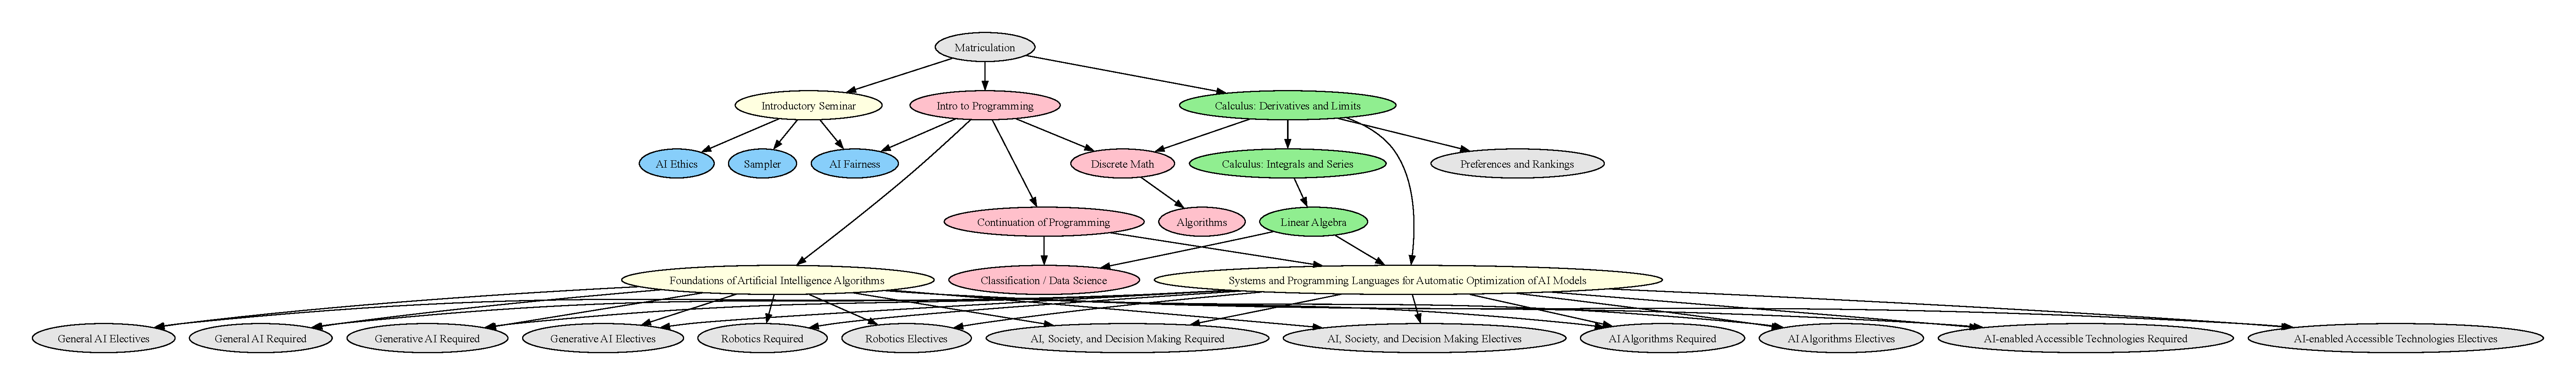
\includegraphics[width=1.2\linewidth]{dependency_graph/all}
  \caption{Dependency graph of the program topics.  Courses created specifically for the \ai{} major in \colorbox{yellow!30}{beige}, interdisciplinary courses in \colorbox{SkyBlue}{blue}, CS courses in \colorbox{red!30}{red}, and math courses in \colorbox{green!30}{green}.}
\end{figure*}


  
%%%%%%%%%%%%%%%%%%%%%%%%%%%%%%%%%%%%%%%%%%%%%%%%%%%%%%
% DO NOT EDIT THIS FILE, IT IS AUTOMATICALLY GENERATED
% INSTEAD, EDIT THE FILE HERE:
%
% https://docs.google.com/spreadsheets/d/1qRaEKxhyfwjHDWa3burGeqK0zeC00Br8NhJfnMWXJdk/edit?usp=sharing
%
% If you edit this file, your changes will be overwritten from this
% spreadsheet linked above.
%%%%%%%%%%%%%%%%%%%%%%%%%%%%%%%%%%%%%%%%%%%%%%%%%%%%%%%
\rowcolors{2}{gray!25}{white}
\begin{longtable}{p{7cm}>{\raggedleft\arraybackslash}p{7cm}}
Topic & Courses \\
\toprule
\textbf{Single Variable Calculus} [4 Credits] & MATH~340 or MATH~140       \\
\textbf{Introductory Seminar} [1 Credits] & AI~101                         \\
\textbf{Intro to Programming} [4 Credits] & CMSC~141, CMSC~131, or INST~326 \\
\textbf{AI's Ethical Frontiers} [3 Credits] & PHIL~211                     \\
\textbf{Multivariable Calculus} [4 Credits] & MATH~141                     \\
\textbf{Sampler} [2 Credits] & AI~102, AI~103, or AI~104                   \\
\textbf{Continuation of Programming} [4 Credits] & CMSC~142 or CMSC~132    \\
\textbf{Discrete Math} [4 Credits] & CMSC~250 or DATA~250                  \\
\textbf{Foundations of Artificial Intelligence Algorithms} [3 Credits] & AI~221 or CMSC~421 \\
\textbf{AI Fairness} [3 Credits] & INST~204                                \\
\textbf{Algorithms} [3 Credits] & CMSC~351                                 \\
\textbf{Linear Algebra} [3 Credits] & MATH~461, DATA~250, MATH~240, MATH~241, or MATH~341 \\
\textbf{Systems and Programming Languages for Automatic Optimization of AI Models} [4 Credits] & \textit{AI~216} \\
\textbf{Classification / Data Science} [3 Credits] & INST~414, CMSC~320, or DATA~320 \\
\textbf{Neural Networks} [3 Credits] & CMSC~472 or AI~372                  \\
\bottomrule
\end{longtable}
Total Credits for Core: 48


\subsection{Interdisciplinary AI Electives}

After completing the core, students can take upper level courses in \ai{} across the curriculum, potentially combining with a minor or certificate.


%%%%%%%%%%%%%%%%%%%%%%%%%%%%%%%%%%%%%%%%%%%%%%%%%%%%%%
% DO NOT EDIT THIS FILE, IT IS AUTOMATICALLY GENERATED
% INSTEAD, EDIT THE FILE HERE:
%
% https://docs.google.com/spreadsheets/d/1qRaEKxhyfwjHDWa3burGeqK0zeC00Br8NhJfnMWXJdk/edit?usp=sharing
%
% If you edit this file, your changes will be overwritten from this
% spreadsheet linked above.
%%%%%%%%%%%%%%%%%%%%%%%%%%%%%%%%%%%%%%%%%%%%%%%%%%%%%%%
\rowcolors{2}{gray!25}{white}
\begin{longtable}{p{7cm}>{\raggedleft\arraybackslash}p{7cm}}
Topic & Courses \\
\toprule
\textbf{General AI Electives} [15 Credits Total] (Take 5 of the courses) & BCHM~477, CHBE~452, CMSC425, CMSC426, CMSC454, CMSC470, CMSC422, CMSC477, CMSC498E, CMSC498Y, ECON~354, ENAE~450, ENAE~488O, ENEE~467, ENMA~437, GEOG398E, GEOG461, IMDM498E, INST461, or PSYC431 \\
\textbf{General AI Required} [3 Credits] & \textit{AI~473}                 \\
\bottomrule
\end{longtable}
Total Credits (including core): 66


\subsection{Specialization: Generative AI}

    Students learn how to build and use, train, and evaluate AIs for generating text, images, and other modalities.

  \rowcolors{2}{gray!25}{white}
\begin{longtable}{p{7cm}>{\raggedleft\arraybackslash}p{7cm}}
Topic & Courses \\
\toprule
\textbf{Gen AI Required} [12 Credits Total] (Take 4 of the courses) & \textit{AI~220}, \textit{AI~370}, LING~200, LING~240, \textit{AI~429}, CMSC~470 \\
\textbf{Gen AI Electives} [6 Credits Total] (Take 2 of the courses) & LING~311, LING~410, CMSC~426, CMSC~427, LING~320, LING~321, LING~322, LING~330 \\
\bottomrule
\end{longtable}
Total Credits (including core): 65


\subsection{Specialization: AI, Society, and Decision Making}


%%%%%%%%%%%%%%%%%%%%%%%%%%%%%%%%%%%%%%%%%%%%%%%%%%%%%%
% DO NOT EDIT THIS FILE, IT IS AUTOMATICALLY GENERATED
% INSTEAD, EDIT THE FILE HERE:
%
% https://docs.google.com/spreadsheets/d/1qRaEKxhyfwjHDWa3burGeqK0zeC00Br8NhJfnMWXJdk/edit?usp=sharing
%
% If you edit this file, your changes will be overwritten from this
% spreadsheet linked above.
%%%%%%%%%%%%%%%%%%%%%%%%%%%%%%%%%%%%%%%%%%%%%%%%%%%%%%%
\rowcolors{2}{gray!25}{white}
\begin{longtable}{p{7cm}>{\raggedleft\arraybackslash}p{7cm}}
Topic & Courses \\
\toprule
\textbf{AI, Society, and Decision Making Required} [12 Credits Total] (Take 4 of the courses) & GEOG~398E, \textit{BSAI~460}, INST~366, or CMSC~401 \\
\textbf{AI, Society, and Decision Making Electives} [6 Credits Total] (Take 2 of the courses) & \textit{BSAI~473}, \textit{BSAI~491}, CMSC~474, WGSS~115, SOCY~100, SOCY~216, SOCY~455, SOCY~456, SOCY~462, PLCY~201, PLCY~215, PLCY~240, BAAI~435, or BAAI~433 \\
\bottomrule
\end{longtable}
Total Credits (including core): 68


\subsection{Specialization: AI Algorithms}


%%%%%%%%%%%%%%%%%%%%%%%%%%%%%%%%%%%%%%%%%%%%%%%%%%%%%%
% DO NOT EDIT THIS FILE, IT IS AUTOMATICALLY GENERATED
% INSTEAD, EDIT THE FILE HERE:
%
% https://docs.google.com/spreadsheets/d/1qRaEKxhyfwjHDWa3burGeqK0zeC00Br8NhJfnMWXJdk/edit?usp=sharing
%
% If you edit this file, your changes will be overwritten from this
% spreadsheet linked above.
%%%%%%%%%%%%%%%%%%%%%%%%%%%%%%%%%%%%%%%%%%%%%%%%%%%%%%%
\rowcolors{2}{gray!25}{white}
\begin{longtable}{p{7cm}>{\raggedleft\arraybackslash}p{7cm}}
Topic & Courses \\
\toprule
\textbf{AI Algorithms Electives} [6 Credits Total] (Take 2 of the courses) & \textit{BSAI~429}, CMSC~426, CMSC~470, CMSC~477, CMSC~401, CMSC~454, or CMSC~426 \\
\textbf{AI Algorithms Required} [12 Credits Total] (Take 4 of the courses) & \textit{BSAI~461}, \textit{BSAI~427}, CMSC~472, or CMSC~422 \\
\bottomrule
\end{longtable}
Total Credits (including core): 68


\subsection{Specialization: Robotics}


%%%%%%%%%%%%%%%%%%%%%%%%%%%%%%%%%%%%%%%%%%%%%%%%%%%%%%
% DO NOT EDIT THIS FILE, IT IS AUTOMATICALLY GENERATED
% INSTEAD, EDIT THE FILE HERE:
%
% https://docs.google.com/spreadsheets/d/1qRaEKxhyfwjHDWa3burGeqK0zeC00Br8NhJfnMWXJdk/edit?usp=sharing
%
% If you edit this file, your changes will be overwritten from this
% spreadsheet linked above.
%%%%%%%%%%%%%%%%%%%%%%%%%%%%%%%%%%%%%%%%%%%%%%%%%%%%%%%
\rowcolors{2}{gray!25}{white}
\begin{longtable}{p{7cm}>{\raggedleft\arraybackslash}p{7cm}}
Course Subject & Courses \\
\toprule
\textbf{Robotics Required} [15 Credits Total] (Take 5 of the courses) & ENME~480, ENAE~450, CMSC~477, ENEE~467, and \textit{\prefix{}~461} \\
\textbf{Robotics Electives} [3 Credits] & ENME~~444, CMSC~422, CMSC~426, CMSC498E, or \textit{\prefix{}~427} \\
\bottomrule
\end{longtable}
Total Credits (including core): 68


\subsection{Additional Specializations}

As AI develops, we will add more specializations (suggestions welcome!).  Of interest are social impact and accessibility.

\section{Relationships}


\subsection{Relationship to AIM}

In Spring 2024, UMD launched the Artificial Intelligence Interdisciplinary Institute at Maryland (AIM), bringing together AI experts across campus to focus on responsible, ethical development and use of the technology to advance public good in industry, government and society. Given the rapid pace of AI development, a core part of AIM’s mission is to reimagine learning in the face of these drastic changes through the introduction of four new interdisciplinary programs, including Bachelor of Science and Bachelor of Arts degrees in Artificial Intelligence. Students across all majors will learn the principles of AI and how they apply to their field of study.

As part of this initiative, \short{} is designed to be an interdisciplinary program from the
ground up and thus will use faculty with joint appointments with
\aim{} and homes for courses to create the new interdisciplinary
courses required for this program.


\subsection{Relationship to Computer Science}

This section outlines how \short{} would be different from the existing computer science degree (with which is shares multiple courses).  The first, consistent with its inclusion in \aim{} is that it's interdisciplinary.  Second, it offers an introduction to \abr{ai} early in students' curriculum.  Finally, it offers another option to help cope with the large demand for computational majors at the University of Maryland.

\paragraph{Interdisciplinary}

At present, the computer science degree (where most students learn the foundations of artificial intelligence) while highly technical, does not require courses in ethics, social issues, or in the foundation of intelligence.
%
Because Maryland is a world leader in these areas and because \abr{ai}'s broad impact on society, future leaders in \abr{ai} will need these softer skills to build effective systems that will benefit society.

Moreover, the interdisciplinary courses offered by \short{} will serve as opportunities to bolster the interdisciplinary research that is a fundamental goal of \aim{}: the coursework and projects that begin in this program can lead to startups, research projects, and synergies across the campus.

\paragraph{Early Onramp}

While there is already an machine learning \abr{ml} concentration within the computer science degree, \abr{ai} courses are locked behind long prerequisite chains (the first course in the current \abr{ml} degree is CMSC 320, and the other \abr{ai}-relevant courses are all 400 level).  
%
By integrating \abr{ai} concepts earlier in the curriculum (starting in the introductory seminar and programming courses), students will be able to see the relevance of \abr{ai} to their interdisciplinary interests.

\paragraph{Complementing Existing Computational Majors}

There is a large demand for computational majors at the University of Maryland.  
%
While computer science and information studies are the largest, there are multiple others.
%
Given the pervasiveness of \abr{ai}, this offers another route: one that offers a rigorous technical component with interdisciplinary connections.\footnote{Of course, there are motivated students that create their own programs that are interdisciplinary (e.g., by double majoring or selecting a minor).  By formalizing these processes, we will both make it easier for more students to build this interdisciplinary path and provide students credentials.}
%
The goal is that having an alternate route will be able to attract students from diverse backgrounds and prepare them for jobs in \abr{ai}. 




\section{How the Program Relates to the State of Maryland}



\subsection{Statewide Need}

The establishment of \name{} directly aligns with Governor Wes Moore's Executive Order 01.01.2024.02, titled ``Catalyzing the Responsible and Productive Use of Artificial Intelligence in Maryland State Government''. This order emphasizes the need for the State to "ensure the use of AI in Maryland state government is responsible, ethical, beneficial, and trustworthy" and acknowledges that ``AI is transforming society and work in myriad ways, and the pace of that change will continue to accelerate''. 

By developing a curriculum that emphasizes responsible AI development and ethical considerations, \short{} will prepare technical graduates to contribute to the State's commitment to "fairness and equity" in AI applications. The program's focus on innovation and human-centered design will support the State's goal to "explore ways AI can be leveraged to improve State services and resident outcomes''---one of the many interdisciplinary applications of \ai{} possible with \short{}. Furthermore, by educating students on privacy, safety, security, and the importance of transparency in AI systems, \short{} will help build a workforce capable of upholding the principles outlined in the Executive Order, ensuring that AI technologies are implemented in ways that are ``valid and reliable'' and that ``preserve individuals' privacy rights''. 

In summary, \short{} will play a pivotal role in fulfilling the directives of the Executive Order by cultivating a skilled workforce dedicated to the responsible and innovative use of AI, thereby supporting Maryland's mission to "Leave No One Behind" in the rapidly evolving technological landscape. 


\subsection{Demand Analysis}

The establishment of \name{} is economically justified by the increasing market demand for artificial intelligence (AI) professionals, particularly in the Washington, D.C. region. While computer science (CS) provides a broad foundation in computing principles, AI focuses on creating intelligent systems capable of tasks that typically require human intelligence, such as learning, reasoning, and problem-solving. This specialization aligns with the distinct skill sets employers want in creating training data for models, evaluating AI models, and adapting existing AI models.

The white paper "From West to the Rest: AI Workforce Trends in the United States," authored by University of Maryland scholars in the Smith School, provides critical insights into the rapidly expanding AI job market. The report highlights that
\begin{quote}
Stripping out the effects of sheer size, AI Jobs Intensity (ratio of AI to all job postings) yields a different picture. Compared to the aggregated US-level AI Jobs Intensity of 0.56\%, Washington DC ranks \#1 at 1.75\%, followed by VA at 1.36\%, with MD not too far behind at 0.83\% (p. 5).
\end{quote}
This is attributed to the region's strong emphasis on defense, public sector applications, and private industries increasingly incorporating AI into their operations. Moreover, the paper notes that 
\begin{quote}
Driving this growth is an all-out embrace of AI by various agencies of the U.S. federal government, including the Department of Defense. As a direct correlate, many of the major equipment, software, and services suppliers to federal agencies and DoD are based in the MD-DC-VA region. These include, among others, Northrop Grumman, Lockheed Martin, Huntington Ingalls, Booz Allen Hamilton, Accenture, and Deloitte. The region is also home to Amazon HQ2 and Capitol One’s corporate HQ (p. 15).\end{quote}
By situating \short{} in this unique economic landscape, the University of Maryland can address a clear market need. The program will prepare graduates with the specialized skills---natural language processing, generative \ai{}, and how to train and adapt models---described in the report, positioning them to thrive in industries that are rapidly adopting AI technologies. This alignment with workforce demands underscores the strategic importance of \short{} in supporting the D.C. region's leadership in AI innovation and implementation.


\subsection{Similar Programs in the State}

To the best of our knowledge, no other institution in the state has an AI degree, although we believe other schools may be developing one.

\subsection{Impact on Historically Black Institutions}


To the best of our knowledge, no other institution in the state has an AI degree, although we believe other schools may be developing one.

\section{Frequently Asked Questions}


\question{Does DATA 250 provide enough of a foundation to satisfy both the linear algebra and discrete math requirements?}

\answer{Waiting on answer\dots}

\question{Will this be an \abr{lep}?}

\answer{Yes, the intention is to submit as an \abr{lep}, although this approval is in some ways parallel to the formal program approval track.}

\question{Why is there no statistics course?}

The committee identified three core skillsets from statistics which are already satisfied in other courses:
\begin{itemize*}
    \item Regression: In multiple courses, most notably CMSC 320
    \item Statistical Tests: In the AI Measurement Course
    \item Inference: In the AI Foundation Course
\end{itemize*}

\question{What is the relationship between CMSC 221 and CMSC 421?  Are they duplicates?}

In the current proposal, we have currently split out the GOFAI course into a higher level one and a lower level one meant for people to take early on in the BS in AI program or as part of some other major.  This is analogous to how Math has a Linear Algebra course for non-majors and one for majors.

How this would actually be implemented is another question.  Perhaps shared lectures and different recitations and homeworks?  Or two completely different courses?  Bill Regli is revampling CMSC 421, and perhaps this could be part of a larger conversation.



  \section{Courses}

In this section, we list the courses used anywhere in the proposal.  The sections are ordered by decreasing changes: new courses first, new courses but already proposed by the \abr{ba} in \abr{ai} (and under development now), followed by existing courses: first those that require slight modifications in delivery of requirements, followed by those used without changes.  

  \subsection{New}

  
%%%%%%%%%%%%%%%%%%%%%%%%%%%%%%%%%%%%%%%%%%%%%%%%%%%%%%
% DO NOT EDIT THIS FILE, IT IS AUTOMATICALLY GENERATED
% INSTEAD, EDIT THE FILE HERE:
%
% https://docs.google.com/spreadsheets/d/1qRaEKxhyfwjHDWa3burGeqK0zeC00Br8NhJfnMWXJdk/edit?usp=sharing
%
% If you edit this file, your changes will be overwritten from this
% spreadsheet linked above.
%%%%%%%%%%%%%%%%%%%%%%%%%%%%%%%%%%%%%%%%%%%%%%%%%%%%%%%
\begin{enumerate}
\item \textbf{Efficient Systems for AI Applications (BSAI 216)}: This course introduces students to the computer system fundamentals that underpin AI systems.  Students learn how memory and parameters are organized in low-level systems and the programming techniques necessary to effeciently update those parameters on large datasets.  Students also learn how the mathematical fundamentals of AI algorithms are translated into learned parameters given large datasets.  Finally, students learn how modern algorithms update those parameters effeciently with large datasets that exceed the capacity of individual computers. [Linear algebra is required for this course but may be taken concurrently.] Prereqs: (Linalg: MATH 240 OR MATH 461 OR DATA 250 OR MATH 243 OR MATH 341 OR ENEE 290) AND (Calc1: MATH 340 OR MATH 140) AND (Programming2: CMSC 142 OR CMSC 132)
\item \textbf{Measuring Preferences and Rankings (BSAI 220)}: A key component of modern AI systems is knowing when one AI system (or its output) is better than another.  Many of the mathematical tools used to make these decisions come from psychology.  This course introduces the mathematical tools that form the foundation of these techniques, teaches students to fit these models to data, and then explains how these models are used in modern AI systems and in AI evaluations. Prereqs: MATH 340 OR MATH 140
\item \textbf{Multilingual Text Processing and Evaluation (BSAI 370)}: This course covers the representation and manipulation of linguistic data on computers.  After establishing the fundamentals of byte-level representation and how different languages are represented on a computer, the course discusses the type / token distinction of word use and how this is reflected in computational representations of language and how this is complicated by languages with implicit or ambiguous tokenization.  Finally, this course covers the application of large models (taken as a given) and resources to novel tasks or in novel combinations: how to adapt existing resources to new tasks, how to evaluate how well the models perform, and how to efficiently adapt models to these tasks.   Prereqs: (Compgraphs: BSAI 216) AND (Gofai: CMSC 421 OR BSAI 221)
\item \textbf{Reinforcement Learning (BSAI 427)}: A survey of the theory and practice of reinforcement learning algorithms: how to formulate reward functions, how to estimate policies given rewards, and how to estimate the value of states given a reward survey.  After introducing the foundations of reinforcement learning, the course covers imitation learning, opponent modeling, and deep Q-learning. Prereqs: (Compgraphs: BSAI 216) AND (Gofai: CMSC 421 OR BSAI 221)
\item \textbf{Multimodal Generation (BSAI 429)}: Introduction to the algorithms that allow the generation of image, sound, video, and other modalities based on instructions, the theory behind joint representations that bridge the divide between description and representation and how they are rendered in the target medium, how to iteratively refine and render the target representations, and how to train and fine-tune the models to be more expressive or cover new concepts.  Discussion of dataset curation, evaluation, detection, and social impact of these algorithms. Prereqs: (Compgraphs: BSAI 216) AND (Gofai: CMSC 421 OR BSAI 221)
\item \textbf{AI and the Life of Great Cities  (BSAI 460)}: "AI, Data Science and Cities" explores the transformative role of artificial intelligence
and data science in shaping urban environments, from smart infrastructure to
data-driven policymaking. Students will learn how to develop and apply AI algorithms
and data science pipelines to enhance mobility, sustainability, and governance while
also considering ethical, social, and equity challenges. Through case studies, hands-on
projects, and interdisciplinary discussions, the course equips students with the technical
and analytical skills needed to design AI- and data-driven urban solutions. By the end,
students will critically assess the potential and limitations of AI and Data Science in
building more resilient, inclusive, and intelligent cities. Prereqs: (Compgraphs: BSAI 216) AND (Gofai: CMSC 421 OR BSAI 221)
\item \textbf{Multiagent Systems (BSAI 461)}: A course on the theory and practice of AI agents interacting in the wild: how to ensure security, how communication protocols can emerge, and how to measure consensus. Prereqs: (Compgraphs: BSAI 216) AND (Gofai: CMSC 421 OR BSAI 221)
\item \textbf{Capstone in Artificial Intelligence (BSAI 473)}: Students will be paired with project advisors from the UMD faculty or alternatively, an industry advisor. Students are encouraged to plan for projects results that can be published at academic conferences or will impact academic research.
Semester-long project course in which each student will identify and carry out a project related to machine learning, with the goal of publishing a research paper or software tool. Prereqs: (Compgraphs: BSAI 216) AND (Gofai: CMSC 421 OR BSAI 221)
\item \textbf{AI Clinic (BSAI 491)}: The AI clinic aims to become the go-to resource for assisting local Maryland
governments and small organizations in their procurement processes for AI tools. The
idea behind the AI Clinic is inspired by legal clinics present across many law schools in
the US as well as by the Clinic to End Tech Abuse (CETA) at Cornell Tech. The AI Clinic
will provide services to local government agencies and small organizations that do not
have the expertise or resources to carry out the evaluation of AI tools that they are
considering using to support their decision-making processes.
The AI Clinic will take on “AI cases” that will be led by one faculty member and by a
group of four students with diverse educational backgrounds. AI cases will provide
semester-long, hands-on learning opportunities for students and will prepare them for
the challenges of AI deployment in real-world settings. The output of the AI cases might
include reports with tool assessments (technical and community-centric) that will be
shared with the agency or organization that requested the case, toolkits for decision
makers on how to carry out their own AI evaluations, or training sessions for decision
makers and small organizations on how to use different types of AI tools, among others. Prereqs: (Compgraphs: BSAI 216) AND (Gofai: CMSC 421 OR BSAI 221)
\end{enumerate}

  \subsection{New, but Shared with BA in AI}

  
%%%%%%%%%%%%%%%%%%%%%%%%%%%%%%%%%%%%%%%%%%%%%%%%%%%%%%
% DO NOT EDIT THIS FILE, IT IS AUTOMATICALLY GENERATED
% INSTEAD, EDIT THE FILE HERE:
%
% https://docs.google.com/spreadsheets/d/1qRaEKxhyfwjHDWa3burGeqK0zeC00Br8NhJfnMWXJdk/edit?usp=sharing
%
% If you edit this file, your changes will be overwritten from this
% spreadsheet linked above.
%%%%%%%%%%%%%%%%%%%%%%%%%%%%%%%%%%%%%%%%%%%%%%%%%%%%%%%
\begin{enumerate}
\item \textbf{User Modeling and Personalization (INST436)}: This would encompass recommender systems (like Netflix recommending movies) and personalization algorithms (like the ones that drive social media feeds). Such systems are a really interesting mix of AI and big data, and are one of the most impactful types of AI that people encounter every day. Prereqs: (Compgraphs: \prefix{} 216) AND (Gofai: \prefix{} 221 OR CMSC 421)
\item \textbf{The Current AI Moment (\prefix{} 101)}: This course introduces students to the current moment of AI.  It introduces the historical analogs of AI (e.g., the upheaval of mechanize agricultural, assembly lines, and information technologies) and compares and contrasts how AI is different.  It provides a non-technical history of the major AI developments of the last hundred years and introduces to societal, ethical, economic, and technical questions that are a part of the AI moment.
\item \textbf{Introduction to AI and the Law (\prefix{} 102)}: This course will examine AI Law and Regulation from the perspective of US Law and industry self-regulation with some discussion of select relevant international law and voluntary frameworks (i.e., EU AI Act and ISO/UN/OECD). Specific topics of US and international law may include: American Legal Process and Procedure, Administrative Law for AI Regulation, Constitutional Law Relationships to AI, Intellectual Property Law (Copyright, Trademark, Patent, and Trade Secret Law), Negligence/Products Liability Law, Privacy Law and Privacy Torts, Fundamentals of Contract Law, Industry Self-Regulation and International Frameworks. Prereqs: \prefix{} 101
\item \textbf{Introduction to AI and Food (\prefix{} 103)}: This course will examine the role of AI in American Food.  From how chemical synthesis driven by AI can produce new fertilizers, insecticides, and other tools that can improve the yield and productivity of crops, to using computer vision to monitor livestock, to harvesting crops with robotic agents, this course will explore the role of AI in food production.  Next, the course will cover the role of AI in food storage, transportation, and its trade on commodities markets.  Finally, the course will end with an overview of AI in food preparation, marketing, and helping individuals making nutritional decisions. Prereqs: \prefix{} 101
\item \textbf{Introduction to AI and Creativity (\prefix{} 104)}: This course will examine the role of AI in creative---particularly visual---pursuits.  Student will learn how to generate and edit images and videos using AI tools and learn the limitations of those tools.  Students will learn how to add additional information to these models and learn how to detect AI-created images and videos.  The final project will be to create a portfolio of artwork assisted by AI tools. Prereqs: \prefix{} 101
\item \textbf{AI and UX (\prefix{} 431)}: The purpose of this course is to teach undergraduate and graduate students how and when to integrate AI-assisted search and validation procedures into their information seeking practices. The course could also be designed to provide UMD with opportunities to collect search results data from low tech student assignments using the AI assisted search engines. Comparing search results year on year could enable researchers to monitor tools as they evolve. The course will also teach students to  compare the information retrieval capabilities of standard search engines to the AI tools and monitor the evolution of both over the semesters. Prereqs: (Compgraphs: \prefix{} 216) AND (Gofai: \prefix{} 221 OR CMSC 421)
\item \textbf{AI and Human Creativity (\prefix{} 432)}: Course will focus on the potential impacts of generative AI systems on human creativity. To do this, students will need to learn about 1) capabilities and limitations of generative AI systems, both currently, and in principle / in the future, and in the context of past work, as well as 2) the human systems (cognitive, social) that produce and govern creative work (broadly construed, including scientific discovery, design, and art and music). Prereqs: (Compgraphs: \prefix{} 216) AND (Gofai: \prefix{} 221 OR CMSC 421)
\item \textbf{Trust, Design, and AI (\prefix{} 433)}: This course will focus on examining how user interfaces are designed for generative AI systems, and how those designs evoke (or fail to evoke) trust in users. Generative AI systems are a main component of our modern society, and at the same time, they are too complex and obscure for users to fully understand. As a result, user interfaces must be designed to make generative AI feel usable, reliable, and trustworthy - whether or not those systems actually are! We’ll examine a variety of user interfaces for generative AI systems, and evaluate their usability, reliability, and trustworthiness. Prereqs: (Compgraphs: \prefix{} 216) AND (Gofai: \prefix{} 221 OR CMSC 421)
\item \textbf{Are Robots Taking our Jobs? (\prefix{} 435)}: Are robots taking our jobs? Are there any jobs even worth taking? What other futures of work might we build? This course examines these questions by focusing on the labor process of computer-supported collaborative work (CSCW) in domains ranging from transportation to software development to sex work, drawing on research and theory from sociology, organizational studies, HCI, and more. Design-oriented students will be encouraged to develop interventions to enhance not just productivity but autonomy and democracy. Research-oriented students will learn to study workplaces and situate shopfloor developments in global political economy. Prereqs: (Compgraphs: \prefix{} 216) AND (Gofai: \prefix{} 221 OR CMSC 421)
\end{enumerate}

    \subsection{Lower Level Alternative to Existing Course}

    Because we want to expose students to AI concepts earlier, we are creating sophomore-level courses that cover similar topics to some of our upper-division courses.  These are not replacing those courses (students could get credit only for one of the two), but providing an alternative (much like math has linear algebra for majors and non-majors).

    
%%%%%%%%%%%%%%%%%%%%%%%%%%%%%%%%%%%%%%%%%%%%%%%%%%%%%%
% DO NOT EDIT THIS FILE, IT IS AUTOMATICALLY GENERATED
% INSTEAD, EDIT THE FILE HERE:
%
% https://docs.google.com/spreadsheets/d/1qRaEKxhyfwjHDWa3burGeqK0zeC00Br8NhJfnMWXJdk/edit?usp=sharing
%
% If you edit this file, your changes will be overwritten from this
% spreadsheet linked above.
%%%%%%%%%%%%%%%%%%%%%%%%%%%%%%%%%%%%%%%%%%%%%%%%%%%%%%%
\begin{enumerate}
\item \textbf{Classical AI Algorithms (\prefix{} 221)}: This course introduces the foundation of AI theory and practice.  Students learn how to search over structured representations to find optimal solutions to planning problems, how to represent real-world problems in graph structures or game trees, and how to represent and solve AI problems using first-order logic.  Credit only granted to one of 421 or 221. Prereqs: INST 326 OR DATA 120 OR CMSC 141 OR CMSC 131
\end{enumerate}

    \subsection{Breadth Courses}

    
%%%%%%%%%%%%%%%%%%%%%%%%%%%%%%%%%%%%%%%%%%%%%%%%%%%%%%
% DO NOT EDIT THIS FILE, IT IS AUTOMATICALLY GENERATED
% INSTEAD, EDIT THE FILE HERE:
%
% https://docs.google.com/spreadsheets/d/1qRaEKxhyfwjHDWa3burGeqK0zeC00Br8NhJfnMWXJdk/edit?usp=sharing
%
% If you edit this file, your changes will be overwritten from this
% spreadsheet linked above.
%%%%%%%%%%%%%%%%%%%%%%%%%%%%%%%%%%%%%%%%%%%%%%%%%%%%%%%
\begin{enumerate}
\end{enumerate}

  \subsection{Refocus}

    Courses already approved and whose material perfectly match the goals of \short{}, but would need to be scaled up.  At the moment, we are also considering allowing the INST introduction to Python (a two course sequence) to substitute for taking CSMC 141.  E.g., students who take the two course INFO programming sequence would be able to continue onto CMSC 142, which focuses on data structures.  The goal is to provide as many pipelines into the program as possible while maintaining rigor.
    
  
%%%%%%%%%%%%%%%%%%%%%%%%%%%%%%%%%%%%%%%%%%%%%%%%%%%%%%
% DO NOT EDIT THIS FILE, IT IS AUTOMATICALLY GENERATED
% INSTEAD, EDIT THE FILE HERE:
%
% https://docs.google.com/spreadsheets/d/1qRaEKxhyfwjHDWa3burGeqK0zeC00Br8NhJfnMWXJdk/edit?usp=sharing
%
% If you edit this file, your changes will be overwritten from this
% spreadsheet linked above.
%%%%%%%%%%%%%%%%%%%%%%%%%%%%%%%%%%%%%%%%%%%%%%%%%%%%%%%
\begin{enumerate}
\item \textbf{Programming with Purpose I: Data-Centric Computing (CMSC 141)}: This course is an introduction to computing and programming through the lens of data. It aims to give you ways of thinking about solving problems using computation. Students will learn to write programs to process both tabular and structured data, to assess programs both experimentally and theoretically, to apply basic data science concepts, and to discuss big ideas around the communication, use, and social impacts of digital information.
\item \textbf{Data Structures and Algorithms (CMSC 142)}: This course explains the concepts and techniques required to write programs that can handle large amounts of data efficiently. Project-oriented and classroom-tested, it presents a number of important algorithms—supported by motivating examples—that bring meaning to the problems faced by computer programmers. The idea of computational complexity is introduced, demonstrating what can and cannot be computed efficiently at scale, helping programmers make informed choices about the algorithms they use.  Prereqs: CMSC 141 OR CMSC 131 OR INST 326
\item \textbf{Privacy, Security and Ethics for Big Data (INST 366)} Prereqs: (Compgraphs: BSAI 216) AND (Gofai: BSAI 221 OR CMSC 421)
\item \textbf{Design and Human Disability and Aging (INST 401 )}: Focuses on the design of consumer products and information systems to enable their use by persons with a wider range of physical, sensory, and cognitive abilities. Overviews aging and major types of impairment as they relate to resulting problems using consumer products and information systems. Focuses on principles of design of mass market products.
\end{enumerate}


    \subsection{Existing, but Need Alternate Prerequisite Structure}

    For courses that require CMSC 216, would allow AI 216 (computational graphs) as an alternative.  For higher-level courses \textbf{NB: These are only AI courses}, we would require AI 221 (AI foundations) instead of CMSC 330 (Organization of Programming Languages).  Of course, the CMSC pathway of 330 would still remain an option.

    
%%%%%%%%%%%%%%%%%%%%%%%%%%%%%%%%%%%%%%%%%%%%%%%%%%%%%%
% DO NOT EDIT THIS FILE, IT IS AUTOMATICALLY GENERATED
% INSTEAD, EDIT THE FILE HERE:
%
% https://docs.google.com/spreadsheets/d/1qRaEKxhyfwjHDWa3burGeqK0zeC00Br8NhJfnMWXJdk/edit?usp=sharing
%
% If you edit this file, your changes will be overwritten from this
% spreadsheet linked above.
%%%%%%%%%%%%%%%%%%%%%%%%%%%%%%%%%%%%%%%%%%%%%%%%%%%%%%%
\begin{enumerate}
\item \textbf{Introduction to Data Science (CMSC 320)}: An introduction to the data science pipeline, i.e., the end-to-end process of going from unstructured, messy data to knowledge and actionable insights. Provides a broad overview of several topics including statistical data analysis, basic data mining and machine learning algorithms, large-scale data management, cloud computing, and information visualization. Prereqs: (Programming2: CMSC 142 OR CMSC 132) AND (Linalg: MATH 240 OR ENEE 290 OR DATA 250 OR MATH 341 OR MATH 243 OR MATH 461)
\item \textbf{Algorithms (CMSC 351)}: A systematic study of the complexity of some elementary algorithms related to sorting, graphs and trees, and combinatorics. Algorithms are analyzed using mathematical techniques to solve recurrences and summations. Prereqs: DATA 250 OR CMSC 250
\item \textbf{Introduction to Artificial Intelligence (CMSC 421)}: Introduces a range of ideas and methods in AI, varying semester to semester but chosen largely from: automated heuristic search, planning, games, knowledge representation, logical and statistical inference, learning, natural language processing, vision, robotics, cognitive modeling, and intelligent agents. Programming projects will help students obtain a hands-on feel for various topics.  Credit only granted to one of 421 or 221.
\item \textbf{Introduction to Machine Learning (CMSC 422)}: Machine Learning studies representations and algorithms that allow machines to improve their performance on a task from experience. This is a broad overview of existing methods for machine learning and an introduction to adaptive systems in general. Emphasis is given to practical aspects of machine learning and data mining. Prereqs: (Compgraphs: BSAI 216) AND (Gofai: CMSC 421 OR BSAI 221)
\item \textbf{Computer Vision (CMSC 426)}: An introduction to basic concepts and techniques in computervision. This includes low-level operations such as image filtering and edge detection, 3D reconstruction of scenes using stereo and structure from motion, and object detection, recognition and classification. Prereqs: (Compgraphs: BSAI 216) AND (Gofai: CMSC 421 OR BSAI 221)
\item \textbf{Computer Graphics (CMSC 427)}: An introduction to 3D computer graphics, focusing on the underlying building blocks and algorithms for applications such as 3D computer games, and augmented and virtual reality (AR/VR). Covers the basics of 3D image generation and 3D modeling, with an emphasis on interactive applications. Discusses the representation of 3D geometry, 3D transformations, projections, rasterization, basics of color spaces, texturing and lighting models, as well as programming of modern Graphics Processing Units (GPUs). Includes programming projects where students build their own 3D rendering engine step-by-step. Prereqs: (Compgraphs: BSAI 216) AND (Gofai: CMSC 421 OR BSAI 221)
\item \textbf{Natural Language Processing (CMSC 470)}: Introduction to fundamental techniques for automatically processing and generating natural language with computers. Machine learning techniques, models, and algorithms that enable computers to deal with the ambiguity and implicit structure of natural language. Application of these techniques in a series of assignments designed to address a core application such as question answering or machine translation.
 Prereqs: (Compgraphs: BSAI 216) AND (Gofai: CMSC 421 OR BSAI 221)
\item \textbf{Introduction to Deep Learning (CMSC 472)}: This course is an elementary introduction to a machine learning technique called deep learning, as well as its applications to a variety of domains. Along the way, the course also provides an intuitive introduction to machine learning such as simple models, learning paradigms, optimization, overfitting, importance of data, training caveats, etc. The assignments explore key concepts and simple applications, and the final project allows an in-depth exploration of a particular application area. By the end of the course, you will have an overview on the deep learning landscape and its applications. You will also have a working knowledge of several types of neural networks, be able to implement and train them, and have a basic understanding of their inner workings. Credit only granted to one of 472 or 372. Prereqs: () AND () AND () AND ()
\end{enumerate}

  \subsection{Existing}

    Existing courses mentioned in the proposal are listed here for completeness (and so readers can look up unfamiliar courses).  

  
%%%%%%%%%%%%%%%%%%%%%%%%%%%%%%%%%%%%%%%%%%%%%%%%%%%%%%
% DO NOT EDIT THIS FILE, IT IS AUTOMATICALLY GENERATED
% INSTEAD, EDIT THE FILE HERE:
%
% https://docs.google.com/spreadsheets/d/1qRaEKxhyfwjHDWa3burGeqK0zeC00Br8NhJfnMWXJdk/edit?usp=sharing
%
% If you edit this file, your changes will be overwritten from this
% spreadsheet linked above.
%%%%%%%%%%%%%%%%%%%%%%%%%%%%%%%%%%%%%%%%%%%%%%%%%%%%%%%
\begin{enumerate}
\item \textbf{(Dis)ability in American Film (AMST 320)}: Explores the connection between film and disability through an analysis of independent and mainstream American films in various film genres. Specifically, we will consider how these film representations reflect and/or challenge the shifting social perspectives of disability over the 20th and 21st centuries. Beginning with the presentation of disability as theatrical spectacle in the traveling sideshow and early cinema, we will work our way through film history to develop an understanding of our society's complicated relationship with disability.
 Prereqs: (\prefix{} 216) AND (\prefix{} 221 OR CMSC 421)
\item \textbf{Object-Oriented Programming I (CMSC 131)}: Introduction to programming and computer science. Emphasizes understanding and implementation of applications using object-oriented techniques. Develops skills such as program design and testing as well as implementation of programs using a graphical IDE. Programming done in Java.
\item \textbf{Object-Oriented Programming II (CMSC 132)}: Introduction to use of computers to solve problems using software engineering principles. Design, build, test, and debug medium -size software systems and learn to use relevant tools. Use object-oriented methods to create effective and efficient problem solutions. Use and implement application programming interfaces (APIs). Programming done in Java.
\item \textbf{Discrete Structures (CMSC 250)}: Fundamental mathematical concepts related to computer science, including finite and infinite sets, relations, functions, and propositional logic. Introduction to other techniques, modeling and solving problems in computer science. Introduction to permutations, combinations, graphs, and trees with selected applications. Prereqs: (MATH 340 OR MATH 140) AND (CMSC 131 OR DATA 120 OR CMSC 141 OR INST 326)
\item \textbf{Algorithms for Geospatial Computing (CMSC 401)}
\item \textbf{Intro to Machine Learning (CMSC 422)}: Machine Learning studies representations and algorithms that allow machines to improve their performance on a task from experience. This is a broad overview of existing methods for machine learning and an introduction to adaptive systems in general. Emphasis is given to practical aspects of machine learning and data mining. Prereqs: () AND () AND () AND () AND ()
\item \textbf{Game Programming (CMSC 425)} Prereqs: (\prefix{} 216) AND (\prefix{} 221 OR CMSC 421)
\item \textbf{Computer Vision (CMSC 426)} Prereqs: (\prefix{} 216) AND (\prefix{} 221 OR CMSC 421)
\item \textbf{Introduction to Human-Computer Interaction (CMSC 434)}: Assess usability by quantitative and qualitative methods. Conduct task analyses, usability tests, expert reviews, and continuing assessments of working products by interviews, surveys, and logging. Apply design processes and guidelines to develop professional quality user interfaces. Build low-fidelity paper mockups, and a high-fidelity prototype using contemporary tools such as graphic editors and a graphical programming environment (eg: Visual Basic, Java).
 Prereqs: (\prefix{} 216) AND (\prefix{} 221 OR CMSC 421)
\item \textbf{Programming Handheld Systems (CMSC 436)}: Fundamental principles and concepts that underlie the programming of handheld systems, such as mobile phones, personal digital assistants, and tablet computers. Particular emphasis will be placed on concepts such as limited display size, power, memory and CPU speed; and new input modalities, where handheld systems differ substantially from non-handheld systems, and thus require special programming tools and approaches. Students will apply these concepts and principles in the context of an existing handset programming platform.
\item \textbf{Algorithms for Data Science (CMSC 454)}: Fundamental methods for processing a high volume of data. Methods include stream processing, locally sensitive hashing, web search methods, page rank computation, network and link analysis, dynamic graph algorithms as well as methods to handle high dimensional data/dimensionality reduction.

\item \textbf{Introduction to Natural Language Processing (CMSC 470)}: Introduction to fundamental techniques for automatically processing and generating natural language with computers. Machine learning techniques, models, and algorithms that enable computers to deal with the ambiguity and implicit structure of natural language. Application of these techniques in a series of assignments designed to address a core application such as question answering or machine translation.
 Prereqs: () AND () AND () AND () AND ()
\item \textbf{Intro to Data Visualization (CMSC 471)}: Datasets are becoming increasingly large and complex, requiring intuitive ways to explore and interpret them quickly and efficiently. In this case, a picture is worth a thousand words: visualizations enable us to transform data into images that are easier to understand and reason about, compared to raw numbers and raw text. Visualizations are critical tools in externalizing and organizing our knowledge and insights, whether to explore collected datasets to improve our understanding of the physical world, to assess and debug analysis/experimental workflows, or to present new and interesting results to diverse audiences. In this course we will study techniques and algorithms for creating effective visualizations based on principles from graphic design, perceptual psychology, and cognitive science. Students will learn how to design and build interactive visualizations for the web, using the D3.js (Data-Driven Documents) framework.
\item \textbf{Introduction to Deep Learning (CMSC 472)}: TEMP Prereqs: (\prefix{} 216) AND (\prefix{} 221 OR CMSC 421)
\item \textbf{Introduction to Computational Game Theory (CMSC 474)} Prereqs: (\prefix{} 216) AND (\prefix{} 221 OR CMSC 421)
\item \textbf{Robotics Perception and Planning (CMSC 477)}: A hands-on introduction to perception and planning for robotics, including rigid body transformations and rotations, dynamics and control of mobile robots/drones, graph based and sampling based planning algorithms, Bayseian and Kalman filtering, camera models and calibration, projective geometry, visual features, optical flow, pose estimation, RANSAC and Hough transform, structure from motion, visual odometry, machine learning basics, visual recognition and learning. Prereqs: () AND () AND ()
\item \textbf{Selected Topics in Computer Science; Robotics (CMSC 498E)}: Overview on fundamental components of robotic systems, including the sensing and actuation, control and modeling of motion and perception, dynamics and kinematics, motion planning and manipulation of robots.
 Prereqs: () AND () AND ()
\item \textbf{Selected Topics in Computer Science; Statistical Inference and Machine Learning Methods for Genomics Data (CMSC 498Y)}: Covers statistical inference and machine learning methods for analyzing genomic data. Examples of topics covered will include maximum likelihood(including composite and pseudo-likelihood functions), expectation-maximization, clustering algorithms, hidden markov models, statistical testing, MCMC and variational inference. Our focus will be on how these techniques are utilized to solve biological problems and the practical challenges that arise when analyzing large genomic data sets.

\item \textbf{Selected Topics in Computer Science; Robotics (CMSC498E)}: Overview on fundamental components of robotic systems, including the sensing and actuation, control and modeling of motion and perception, dynamics and kinematics, motion planning and manipulation of robots. Prereqs: () AND () AND ()
\item \textbf{Object-Oriented Programming I (DATA 120)}:  An introduction to programming in Python language, using Jupyter Notebooks and Python scripts. Covers variables, conditionals, loops, functions, lists, strings, tuples, sets, dictionaries, files and visualization.
\item \textbf{Discrete Mathematics (DATA 250)}: The art and science of discrete mathematics (not Calculus) and rigorous arguments related to
programming and data. Logic, set theory, and formal proofs will be covered in the first portion of the
course, and the second portion will be basic linear algebra, including matrices and systems of equations.
Emphasis on examples and applications so there will be some programming and other uses of the
computer. Classtime consists of lectures, group work, and other classwork. Prereqs: (MATH 340 OR MATH 140) AND (CMSC 131 OR DATA 120 OR CMSC 141 OR INST 326)
\item \textbf{Introduction to Data Science (DATA 320)}: An introduction to data science i.e., the end-to-end process of going from unstructured, messy data to knowledge and actionable insights. Provides a broad overview of several topics including statistical data analysis, basic data mining and machine learning algorithms, large-scale data management, cloud computing, and information visualization.
\item \textbf{Robotics Programming (ENAE 450)}: This practical robotics class teaches practical skills to build, control, and deploy robotic systems. Interdisciplinary groups of students develop real-world robotic systems. The first 10 weeks of the lab are devoted to 5 pre-programmed experiments. The remainder of the lab is devoted to student projects. Students work in teams of 2, preferably with each student coming from a different background in engineering. There are 2 weekly lectures. The emphasis of the class is entirely on making a real robot do what you want it to do. In the first experiment, students perform a simple servomechanism experiment, where students control a single joint of a robot. We vary the weight on the movable rod to simulate the effects of the changing inertia due to outer segments moving. Next, we have the students directly control several joints of a robot arm. The third experiment is to control the position and orientation of the end effector. A fourth experiment deals with grasping. A fifth experiment deals with the position and orientation of a wheeled robot. 
\item \textbf{Introduction to Differential Equations and Linear Algebra for Engineers (ENEE 290)}: First-order differential equations, matrices and systems of linear equations, finite-dimensional vector spaces, inner product spaces, eigenvalues and eigenvectors, linear differential equations of higher order, and systems of differential equations. This course covers important topics in mathematics for Electrical and Computer Engineers. Specifically, several topics are covered, including first-order differential equations, matrices and systems of linear equations, finite-dimensional vector spaces, inner product spaces, eigenvalues and eigenvectors, linear differential equations of higher order, and systems of differential equations. Theoretical topics presented in the lectures will be reinforced by laboratory exercises.

\item \textbf{Robotics Project Laboratory (ENEE 467)}: This practical robotics class teaches practical skills to build, control, and deploy robotic systems. Interdisciplinary groups of students develop real-world robotic systems. The first 10 weeks of the lab are devoted to 5 pre-programmed experiments. The remainder of the lab is devoted to student projects. Students work in teams of 2, preferably with each student coming from a different background in engineering. There are 2 weekly lectures. The emphasis of the class is entirely on making a real robot do what you want it to do. In the first experiment, students perform a simple servomechanism experiment, where students control a single joint of a robot. We vary the weight on the movable rod to simulate the effects of the changing inertia due to outer segments moving. Next, we have the students directly control several joints of a robot arm. The third experiment is to control the position and orientation of the end effector. A fourth experiment deals with grasping. A fifth experiment deals with the position and orientation of a wheeled robot. 
\item \textbf{Assistive Robotics (ENME  444)}: Fundamentals of assistive robots used in a wide varietyof ways to help humans with disabilities. Three application areas will be covered: (1) Rehabilitation robotics to recover motor function from neurologic injuries such as stroke, (2) Prosthetics to enable mobility function in amputees, and (3) Social robotics for cognitive impairment and developmental disorders such as autism. Theory behind different control systems employed by assistive robotics, as well as the mechanical design, sensors, and actuators, and user interfaces behind representative robots in the respective areas. Guidelines for designing assistive robots. Ethical and regulatory considerations in the design of assistive robots.
\item \textbf{Introduction to Robotics (ENME 480)}: This course is an introductory course to the robotics minor and educates students in the elementary concepts of robotics. The topics covered in the course include mathematics of rigid motion, rotations, translations, homogeneous transformations, forward kinematics, inverse kinematics, velocity kinematics, geometric Jacobian, analytical Jacobian, motion planning, trajectory generation, independent joint control, linear control methods such as PD, PID, actuator dynamics, feedforward control for trajectory tracking, force control, basic computer vision concepts including thresholding, image segmentation, and camera calibration. This course also includes a laboratory component to be conducted in the Robot Realization Laboratory in the Engineering Annex Building. Prereqs: () AND () AND ()
\item \textbf{Special Topics in Geography; Introduction to Spatial Artificial Intelligence (GEOG 398E)}: An introductory course to spatial artificial intelligence (AI), providing a big picture of spatial AI applications (e.g., Google Maps, Uber/Lyft, Earth observation, smart cities, autonomous vehicles), techniques, platforms, trends, debates, etc. The course will cover basics of AI, identify challenges faced by AI techniques in the context of spatial data and applications, and introduce spatial-aware AI methods to address them. AI topics include but are not limited to: spatial data models and knowledge representation, pattern mining, machine learning, perception, planning, etc. Students are expected to have a broad understanding of spatial A concepts, develop intuitions and insights to AI techniques, and have some hands-on experience (Python) at the end of the course. Prereqs: (\prefix{} 216) AND (\prefix{} 221 OR CMSC 421)
\item \textbf{Special Topics in Immersive Media; Creative Experiments with AI (IMDM 498E)} Prereqs: (\prefix{} 216) AND (\prefix{} 221 OR CMSC 421)
\item \textbf{Designing Fair Systems (INST 204)}: Reviews how specific values are built into different automated decision-making systems as an inevitable result of constructing mechanisms meant to produce specific outcomes. These values create differential outcomes for the different people enmeshed in these systems, but both these values and these systems can be changed to support different values and different outcomes. The class serves as an introduction to the emerging field of algorithmic bias that bridges the disciplines of information science, computer science, law, policy, philosophy, sociology, urban planning, and others. Prereqs: (\prefix{} 101) AND (CMSC 131 OR DATA 120 OR CMSC 141 OR INST 326)
\item \textbf{Object-Oriented Programming for Information Science (INST 326)}: An introduction to programming, emphasizing understanding and
implementation of applications using object-oriented techniques. Topics to
be covered include program design and testing as well as implementation of
programs.
\item \textbf{User-Centered Design (INST 362)}: Introduction to human-computer interaction (HCI), with a focus on how HCI connects psychology, information systems, computer science, and human factors. User-centered design and user interface implementation methods discussed include identifying user needs, understanding user behaviors, envisioning interfaces, and utilizing prototyping tools, with an emphasis on incorporating people in the design process from initial field observations to summative usability testing.

\item \textbf{Designing Patient-Centered Technologies (INST 402)}: Companies have created a vast array of apps and other technologies for understanding managing personal health and wellness, but many of them have been created with little understanding of audience needs or potential ethical issues. Course introduces students to the unique challenges of studying people's health and wellness needs as well as designing and evaluating technologies to meet those needs.
\item \textbf{Data Science Techniques (INST 414)}: An exploration of how to extract insights from large-scale datasets. The course will cover the complete analytical funnel from data extraction and cleaning to data analysis and insights interpretation and visualization. The data analysis component will focus on techniques in both supervised and unsupervised learning to extract information from datasets. Topics will include clustering, classification, and regression techniques. Through homework assignments, a project, exams and in-class activities, students will practice working with these techniques and tools to extract relevant information from structured and unstructured data. Prereqs: () AND () AND () AND () AND () AND () AND () AND () AND () AND () AND ()
\item \textbf{Emerging Technologies and Risk Management (INST 461)} Prereqs: (\prefix{} 216) AND (\prefix{} 221 OR CMSC 421)
\item \textbf{Introductory Linguistics (LING 200)}: An exploration of the nature of human language. Introduction to the basic concepts and methodology of modern linguistic analysis (sound systems, word formation, sentence structure). Examination of the factors that contribute to dialect differences and the social implications of language variation. Additional topics may include: semantics, pragmatics, language change, writing systems, typology, language universals, comparison with other communication systems. Prereqs: (\prefix{} 216) AND (\prefix{} 221 OR CMSC 421)
\item \textbf{Language and Mind (LING 240)}: The study of language as a cognitive phenomenon. Ways of representing people's knowledge of their native language, ways in which that knowledge is attained naturally by children, and how it is used in speaking and listening. Additional topics may include: animal communication, language and the brain, language and thought. Prereqs: (\prefix{} 216) AND (\prefix{} 221 OR CMSC 421)
\item \textbf{Syntax I (LING 311)}: Basic concepts, analytical techniques of generative syntax, relation to empirical limits imposed by viewing grammars as representations of a component of human mind. Aspects of current theories.
\item \textbf{Phonetics (LING 320)}: Representations and models of acoustic and articulatory phonetics. Develops concepts and skills for description, measurement and scientific analysis of the sound systems of human languages, including various varieties of English.

\item \textbf{Phonology I (LING 321)}: Properties of sound systems of human languages, basic concepts and analytical techniques of generative phonology. Empirical limits imposed by viewing grammars as cognitive representations. Physiological properties and phonological systems; articulatory phonetics and distinctive feature theory.
\item \textbf{Phonology II (LING 322)}: Continuation of LING321. Further investigation of phonological phenomena and phonological theory. Revising and elaborating the theory of the phonological representation; interaction of phonology and morphology.
\item \textbf{Grammar and Meaning (LING 410)}: The basic notions of semantic theory: reference, quantification, scope relations, compositionality, thematic relations, tense and time, etc. The role these notions play in grammars of natural languages. Properties of logical form and relationship with syntax.
\item \textbf{Child Language Acquisition (LING 444)}: Examines language acquisition in infancy and early childhood: the nature of children's linguistic representations and how these develop naturally. Role of (possible) innate linguistic structure and interaction of such structure with experience. Evaluation of methods and results of current and classic research leading to contemporary models of language development.
\item \textbf{Calculus I (MATH 140)}: Introduction to calculus, including functions, limits, continuity, derivatives and applications of the derivative, sketching of graphs of functions, introduction to definite and indefinite integrals, and calculation of area. The course is especially recommended for science and mathematics majors. Credit will be granted for only one of the following: MATH 140 or MATH 136 or MATH 120.
\item \textbf{Calculus II (MATH 141)}: Continuation of MATH140, including techniques of integration, improper integrals, applications of integration (such as volumes, work, arc length, moments), inverse functions, exponential and logarithmic functions, sequences and series.
\item \textbf{Introduction to Linear Algebra (MATH 240)}: Basic concepts of linear algebra: vector spaces, applications to line and plane geometry, linear equations and matrices, similar matrices, linear transformations, eigenvalues, determinants and quadratic forms. All sections of the course will use the software system MATLAB. Credit will be granted for only one of the following: MATH 240 or MATH 341 or MATH 461.
\item \textbf{Introduction to Linear Algebra and Differential Equations (MATH 243)}: The basics of linear algebra and differential equations, with an emphasis on general physical and
engineering applications. Aimed at students who need the material for future coursework but do not
need as much depth and rigor as provided by MATH240/MATH461 and MATH246.
\item \textbf{Multivariable Calculus, Linear Algebra and Differential Equations I (Honors) (MATH 340)}: This is the first semester of the two-semester honors sequence Math 340-341 which gives a unified and enriched treatment of multivariable calculus, linear algebra, and ordinary differential equations, with supplementary material from differential geometry, Fourier series and calculus of variations.
\item \textbf{Multivariable Calculus, Linear Algebra and Differential Equations II (MATH 341)}: This course is a continuation of MATH 340. The honors sequence MATH 340-341 covers roughly the same material of MATH 240, 241, and 246, but in greater depth and rigor. This semeseter will begin with remaining material from Multivariable Calculus (MATH 241) on extrema of functions of several variables and Lagrange multipliers. The remainder of the semester, and the bulk of the course, is then devoted to the theory of Ordinary Differential Equations (MATH 246).
\item \textbf{Linear Algebra for Scientists and Engineers (MATH 461)}: The course provides an introduction to linear algebra and matrix theory. It is intended primarily for engineering students. This course cannot be used toward the upper level math requirements for MATH/STAT majors. Credit will be granted for only one of the following: MATH 240, MATH 341, or MATH 461.
\item \textbf{AI and Ethics (PHIL 211)}: An introduction to a major subfield of contemporary Philosophy, namely applied ethics, and the experience of using some major tools in the practice of philosophy more generally, namely, the construction and formal evaluation of arguments, conceptual analysis, the use of thought experiments, and clear, direct and persuasive writing. Learning how to execute the latter will involve an intense iterative process.
The substantive focus of the course will be the ethical evaluation of AI in some of its current and potentially future incarnations. We’ll examine algorithmic opacity, algorithmic bias
and decision-making, autonomous weapons systems, human-robot interaction, and artificial
moral agents, in order to uncover what, if any, ethical issues they give rise to. Prereqs: \prefix{} 101
\item \textbf{Public Leaders and Active Citizens (PLCY 201)}: Aims to inspire, teach and engage students in the theory and practice of public leadership from the local to the national to the global level. Students will learn and apply diverse approaches to leadership in a multicultural society while developing an understanding of key frameworks and practices necessary to foster collective action across private, public, and nonprofit sectors. This course will allow students to become informed citizens able to reason critically and persuasively about public matters Students will also explore and assess their own personal values, beliefs, and purpose as they develop their leadership potential. Prereqs: (\prefix{} 216) AND (\prefix{} 221 OR CMSC 421)
\item \textbf{Innovation and Social Change: Creating Change for Good (PLCY 215)}: A team-based, highly interactive and dynamic course that provides an opportunity for students to generate solutions to a wide range of problems facing many communities today. Students in the iGIVE Program will deepen their understanding of entrepreneurship and innovation practices by creating and implementing projects or ventures that address an issue of their choosing while learning topics such as communications, project management, teamwork, leadership, fundraising, project sustainability and next steps in social change. Prereqs: (\prefix{} 216) AND (\prefix{} 221 OR CMSC 421)
\item \textbf{Ethical, Policy and Social Implications for Science and Technology (PLCY 240)}: Asks students to think about how society should manage complexity, transformation, and uncertainty with an eye on developing a broader sense of ethics and social responsibility. Introduces analytical frameworks, concepts, and data collection techniques that interdisciplinary scholars use to map relationships among science, technology and society and generate important questions about the future of society. Prereqs: (\prefix{} 216) AND (\prefix{} 221 OR CMSC 421)
\item \textbf{Human and Animal Intelligence (PSYC 431)}: The study of intelligence touches upon a broad range of topics from cognition, animal behavior, philosophy, psychology, and linguistics. Through lectures, discussions, and critical evaluation of opposing arguments, we will investigate the construct of intelligence from an evolutionary perspective. An understanding of animal intelligence also has important applications for understanding cognition in general, the design of robotic controls, investigating human health, conserving endangered species, development of artificial intelligence, and assuring animal welfare.
\item \textbf{Introduction to Sociology (SOCY 100)}: Introduces fundamental concepts and theories of sociology. Guided by C. Wright Mills' "sociological imagination," the course promotes critical thinking; challenges conventional assumptions about culture politics, history, and psychology; and equips students with theoretical approaches and research methods to analyze various sociological topics, including family, work, education, religion, social movements, and issues related to class, gender, race, and ethnic inequalities. Prereqs: (\prefix{} 216) AND (\prefix{} 221 OR CMSC 421)
\item \textbf{Social Aspects of Artificial Intelligence (SOCY 216)}: In two generations computers insinuated themselves into the way societies create wealth, wage war, work, and govern their citizens. While scientists across disciplines debate the feasibility of engineering artificial general intelligence, the race is on to create computers (classic and quantum) that match or surpass human intelligence in as many domains as possible. Students in this course will weigh some social consequences of living with smart machines that are everywhere and never sleep, and confront the question of whether AI has gone too far, or not far enough. Prereqs: (\prefix{} 216) AND (\prefix{} 221 OR CMSC 421)
\item \textbf{Social Dimensions of Privacy and Surveillance (SOCY 455)}: Today, it is quite common in many spheres of life that we divulge personal information in exchange for something else. This course examines practices of surveillance in contemporary society in relationship to collective understandings of privacy. By the end of this course, students will be able to analyze privacy norms and practices in the age of mass surveillance, how surveillance produces inequalities in relation to privacy, and how definitions and regulations of privacy and surveillance change over time.
\item \textbf{Smart Machines and Human Prospects (SOCY 456)}: Artificial intelligence is everywhere and never sleeps. It is transforming our social institutions in intended and unintended ways. While scientists debate the feasibility of engineering conscious machines with general intelligence, no one debates that the global race is on to create more potent computers. Through targeted research, discussion, and presentation of findings students will answer a specific question on how, where, and in what ways society is being changed by smart machines.
\item \textbf{Digital Technology and Society (SOCY 462)}: Situates digital technology in our social environment and then examines how this relationship reflects, reinforces, or reorders social hierarchies. Students will learn the conceptual and methodological foundations for studying and evaluating how technologies such as health and social media apps, the personal computer, artificial intelligence, and weapons of war have evolved, diffused and impacted social life. Students will explore and then conduct independent research on the relationship between technology and social inequalities through the lens of health and medicine, the environment and climate change, jobs and the workplace, as well as government and criminal justice.
\item \textbf{Applied Probability and Statistics I (STAT 400)}: Stat 400 is an introductory course to probability, the mathematical theory of randomness, and to statistics, the mathematical science of data analysis and analysis in the presence of uncertainty. Applications of statistics and probability to real world problems are also presented. Prereqs: MATH 340 OR MATH 140
\item \textbf{Introduction to Data Science and Machine Learning (STAT 426)}: An introductory course to the recent developments in the fields of data science and machine learning. Emphasis will be given to mathematical and statistical understanding of commonly used methods and processes.
 Prereqs: () AND ()
\item \textbf{Introduction to Disability Studies (WGSS 105)}: This course will introduce students to theories of disability justice as they intersect with feminist and antiracist struggles. Tracing the emergence of the concept of disability alongside the rise of racial knowledge since the 19th century, we will consider how disability activists have responded to ableism by developing art, political strategies, and subcultures that promote a more just society built for a wider variety of human bodies. Students will learn about the moral, medical, social, and ecological models of disability; explore varied disability experiences relating to mental illness, chronic disease, and sensory and mobility impairments; debate ethical questions concerning eugenics, selective abortion, health care access, and medical technologies; and analyze the work of disabled artists and activists of color. Students will also discuss principles of universal design which seek to make classrooms more just and collaborative. In order to balance accessibility and community building, the course has been designed for synchronous online instruction complemented by optional in-person sessions.
 Prereqs: (\prefix{} 216) AND (\prefix{} 221 OR CMSC 421)
\item \textbf{Gender, Race and Computing (WGSS 115)}: Race and gender have shaped computing from its earliest histories to contemporary debates over bias in search algorithms, surveillance, and AI. As computational processes shape ever more dimensions of everyday life from the personal to the global scale, understanding how they operate and how power operates within them grows ever more important. Combating racism and sexism is not as simple as ensuring the pool of programmers and engineers is more diverse; structures of power are embedded in digital technologies as they are in all aspects of our society, and we must learn to perceive their operation if we hope to transform them. We will examine how racism and sexism operate in the field of computer science and in everyday uses of digital technologies, while studying how feminist and racial justice movements have created alternative approaches. This class is for anyone who wishes to better understand the relationships between digital technology, structural power, and social justice.

\end{enumerate}
  
  
\section{Library Collection Assessment for BS in Artificial Intelligence}


\subsection*{To:}
CS Department; Artificial Intelligence Interdisciplinary Institute at Maryland (AIM)\\
Jordan Lee Boyd-Graber, Department of Computer Science; Institute of Advanced Computer Studies; iSchool; Language Science Center\\
Neda Atanasoski, Chair, Department of Women, Gender, and Sexuality Studies; AIM Associate Director of Education\\
Matthias Zwicker, Chair, Department of Computer Science

\subsection*{From:}
On behalf of the University of Maryland Libraries:\\
Nevenka Zdravkovska, Head, STEM Library; Library Subject Liaison for Physics and Astronomy\\
Kapil Vasudev, Collection Development Strategies Librarian\\
Maggie Saponaro, Director, Collection Development Strategies\\
Daniel Mack, Associate Dean of Libraries, Collection Strategies \& Services and Interim Dean of Libraries

\subsection*{Subject:}
Library Collection Assessment BS in Artificial Intelligence

\subsection*{Introduction}
We are providing this assessment in response to a proposal by the Artificial Intelligence Interdisciplinary Institute at Maryland (AIM) in the Department of Computer Science to create a BS in Artificial Intelligence program. The Artificial Intelligence Interdisciplinary Institute at Maryland (AIM) asked that we at the University of Maryland Libraries assess our collection resources to determine how well the Libraries support the curriculum of this proposed program.

\subsection*{Serial Publications}
The University of Maryland Libraries currently subscribe to a large number of scholarly journals—almost all in online format—that focus on artificial intelligence.\\
The Libraries subscribe to most of the top-ranked journals that are listed in the Computer Science, Artificial Intelligence category in the 2023 Science Edition of Journal Citation Reports. These journals include the following, all of which are available online:

\begin{itemize}
    \item Foundations and Trends in Machine Learning
    \item IEEE Transactions on Pattern Analysis and Machine Intelligence
    \item Nature Machine Intelligence
    \item Information Fusion
    \item IEEE Transactions on Intelligent Vehicles
    \item IEEE Transactions on Evolutionary Computation
    \item International Journal on Computer Vision
    \item IEEE Transactions on Image Processing
    \item IEEE Transactions on Fuzzy Systems
    \item Medical Image Analysis
    \item Artificial Intelligence Review
    \item IEEE Computational Intelligence Magazine
    \item IEEE Transactions on Neural Networks and Learning Systems
    \item IEEE Transactions on Affective Computing
    \item Energy and AI
\end{itemize}

The highly-ranked core journal to which the Libraries do not currently subscribe is \textit{Foundations and Trends in Machine Learning} published by Now Publisher. However, articles in journals that we do not own likely will be available through Interlibrary Loan/Document Delivery.\\
\textbf{AI research in general is very transparent}, and most publications are accessible to the general public without a subscription, including:

\begin{itemize}
    \item NeurIPS - Neural Information Processing Systems
    \item JMLR - Journal of Machine Learning Research
    \item ACL Publications (EMNLP, ACL, NAACL, etc.)
    \item ICML - International Conference on Machine Learning
    \item UAI - Uncertainty in Artificial Intelligence
    \item ICLR - International Conference on Learning Representations
    \item TACL - Transactions of the Association for Computational Linguistics
    \item CL - Computational Linguistics
\end{itemize}

\subsection*{Databases}
The Libraries’ \href{https://lib.guides.umd.edu/az.php}{Database Finder} offers online access to databases that provide indexing and access to scholarly journal articles and other information sources. Relevant databases include:
\begin{itemize}
    \item ACM
    \item IEEE Xplore
    \item Agricola
    \item Medline
    \item Philosopher's Index with Full Text
    \item ScienceDirect
    \item Multidisciplinary databases: Academic Search Ultimate, Scopus, Web of Science
\end{itemize}

\subsection*{Monographs}
The Libraries regularly acquire scholarly monographs in artificial intelligence and allied disciplines. A search of the University of Maryland Libraries’ UMD Discover catalog yielded sizable lists of citations of books that we own. Below is a sample of the results:

\begin{table}[h!]
\centering
\begin{tabular}{|l|r|r|}
\hline
\textbf{Search Terms} & \textbf{UMD Holdings} & \textbf{Worldwide Holdings} \\
\hline
Artificial Intelligence OR AI & 30,791 & 874,094 \\
Artificial Intelligence OR AI AND ethic* & 15,687 & 165,503 \\
Artificial Intelligence OR AI AND irrigat* & 15,177 & 161,164 \\
\hline
\end{tabular}
\caption{UMD Discover Advanced Sample Searches}
\end{table}

\subsection*{Conclusion}
With our journal holdings, monographs, and databases, as well as additional support services and resources, at this point in time, our assessment is that the University of Maryland Libraries are able to meet the curricular and research needs of the proposed BS in Artificial Intelligence.\\
However, given the challenges of resource inflation costs and finite budget allocation, the Libraries cannot guarantee that we will continue to have access to these resources in the near future.


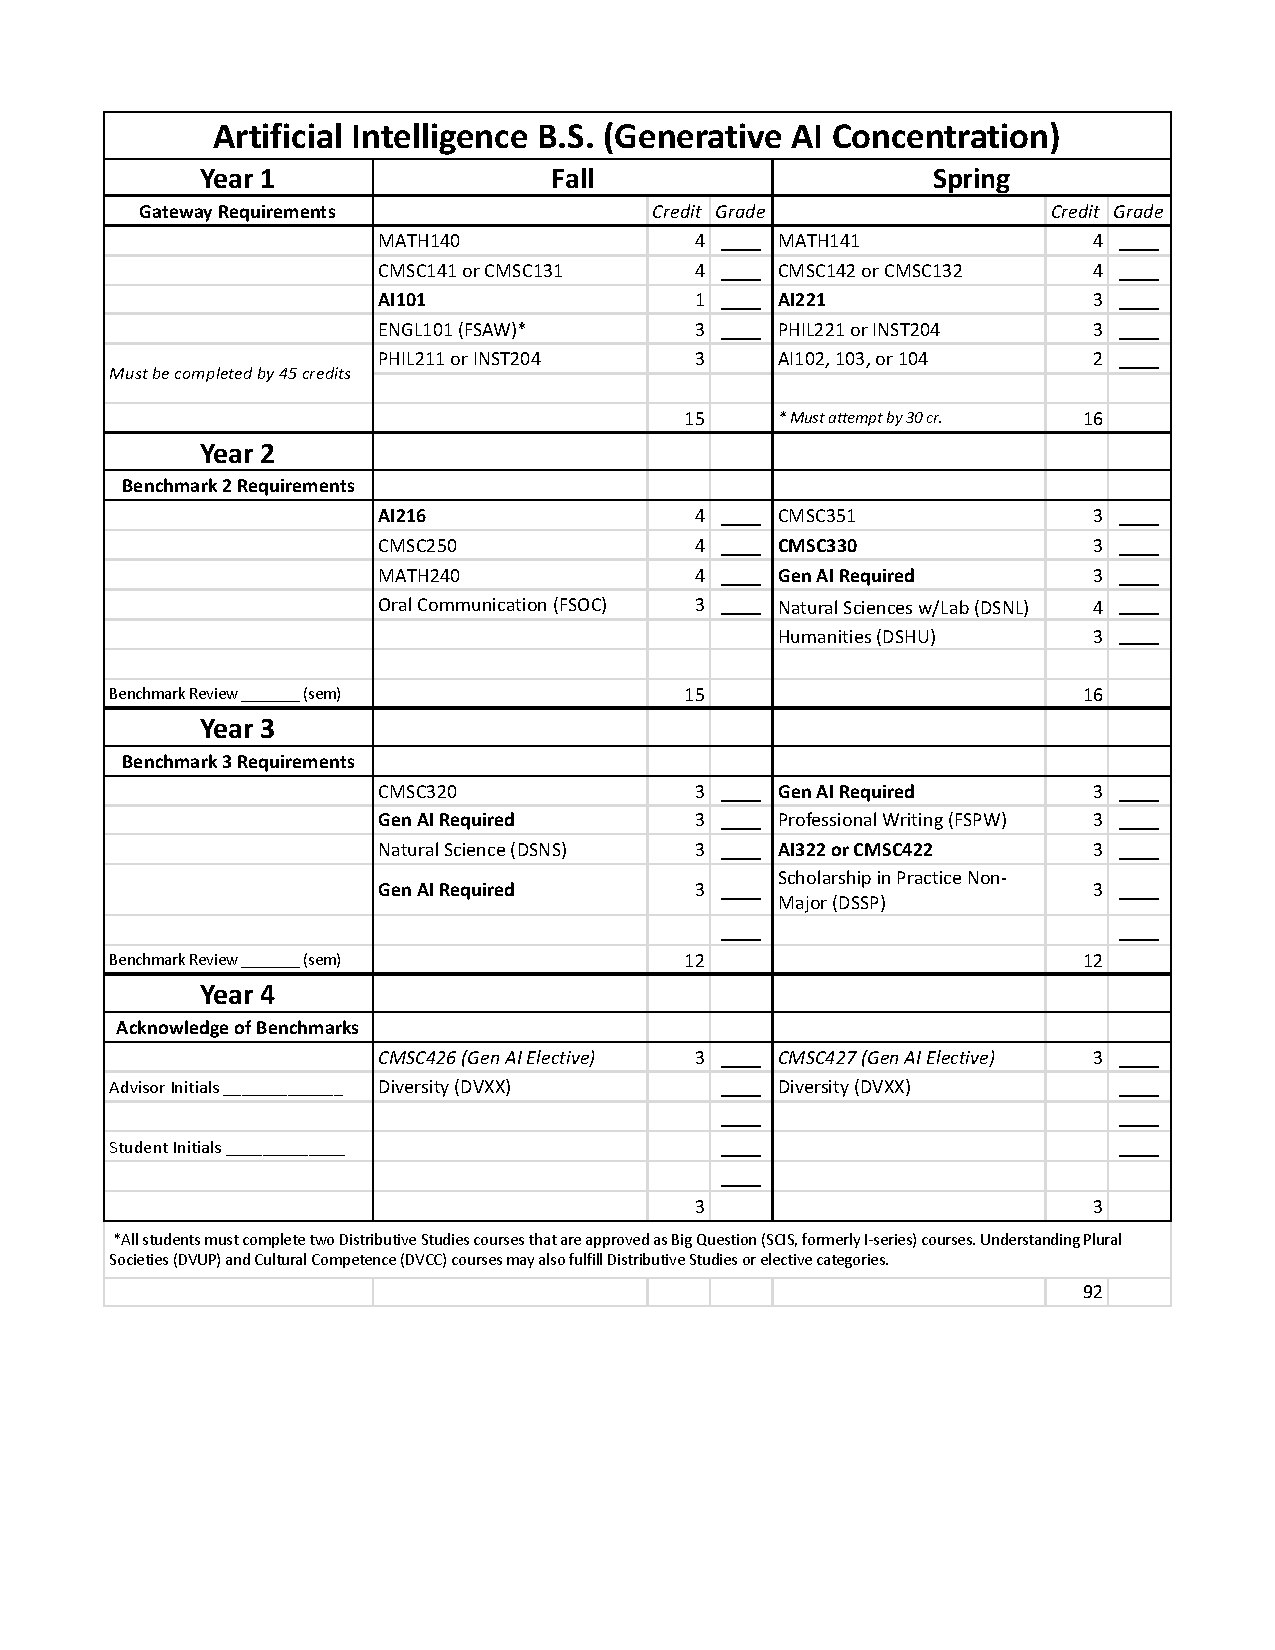
\includepdf[fitpaper=true, pages=-]{schedules/GenAI}

% \begin{definition}[Gauss] 
% To a mathematician it is obvious that
% $\int_{-\infty}^{+\infty}
% e^{-x^2}\,dx=\sqrt{\pi}$. 
% \end{definition} 

% \begin{theorem}[Pythagoras]
% The square of the hypotenuse (the side opposite the right angle) is equal to the sum of the squares of the other two sides.
% \end{theorem}

% \begin{proof} 
% We have that $\log(1)^2 = 2\log(1)$.
% But we also have that $\log(-1)^2=\log(1)=0$.
% Then $2\log(-1)=0$, from which the proof.
% \end{proof}

%----------------------------------------------------------------------------------------
%	BIBLIOGRAPHY
%----------------------------------------------------------------------------------------

% \renewcommand{\refname}{\spacedlowsmallcaps{References}} % For modifying the bibliography heading

% \bibliographystyle{unsrt}

% \bibliography{sample.bib} % The file containing the bibliography

%----------------------------------------------------------------------------------------

\end{document}
